
\documentclass[a4paper,12pt]{article}
\usepackage[unicode,colorlinks=false]{hyperref}


\usepackage[utf8x]{inputenc}
%

\usepackage[L7x]{fontenc}
\usepackage{times}
\usepackage{ucs}

 %package to switch the language
\usepackage{etoolbox}

  %set up of the page margins
\usepackage[top=2cm, bottom=2cm, left=3cm, right=1.5cm]{geometry}

 %1.1 line spacing
\linespread{1.1}


  %page numbering at the right side
\usepackage{fancyhdr}
\pagestyle{fancyplain}
\fancyhf{}
\renewcommand{\headrulewidth}{0pt} 
\fancyhfoffset[RO]{0cm}

  %to number at the bottom (exchange lines to number at the top)
\rfoot{\thepage}
  %\rhead{\thepage} %

% \usepackage[usenames,dvipsnames]{pstricks}
\urlstyle{same}
\hypersetup{
%  citecolor=Blue,
%  linkcolor=Blue,
%  urlcolor=Blue
pdfborder={0 0 0 }
}

 %for includegraphics
\usepackage{graphicx}



\usepackage[toc,page]{appendix}


\usepackage{caption}

 %for source codes
\usepackage{listings}
\lstset{commentstyle=\color{red},xleftmargin=10pt, framexleftmargin=6pt, numbersep=1mm, frame=single, numbers=left,numberstyle=\footnotesize,extendedchars=\true, inputencoding=utf8x,basicstyle=\footnotesize,extendedchars=true,
 keywordstyle=\color{black}\bfseries, breaklines=true, breakautoindent=true,framesep=8pt,linewidth=0.95\textwidth
}

 %for algorithms
\usepackage{algorithm}
\usepackage{algorithmic}
 %instead of the above two packages we can use algorithms2e
 %\usepackage[boxed,linesnumbered,vlined,slide]{algorithm2e}

 %special symbols
\usepackage{amsfonts}
\usepackage{amssymb}
\usepackage{amsmath}

 %for theorem like environments
\usepackage{amsthm}

 \usepackage{datetime}
 \renewcommand{\dateseparator}{--}


% SI system units
\usepackage{siunitx}
\sisetup{detect-all}
% Problem with fonts \SI{x.xx}{\micro\metre}, solved with updmap-sys --enable Map=utm.map
\renewcommand{\sfdefault}{uhv}
\renewcommand{\rmdefault}{utm}
\renewcommand{\ttdefault}{ucr}

% List management (itemize, etc.)
\usepackage{enumitem}

\newcommand*{\urlw}[1]{\href{#1}%
            {\nolinkurl{#1}}}

\numberwithin{equation}{section}


\newtoggle{inLithuanian}
 %If the report is in Lithuanian, it is set to true; otherwise, change to false
\settoggle{inLithuanian}{true}

%create file preface.tex for the preface text
\newtoggle{needPreface}
\settoggle{needPreface}{false}

\newtoggle{signaturesOnTitlePage}
\settoggle{signaturesOnTitlePage}{false}


\theoremstyle{definition}
\newtheorem{definition}{\keyWordDefinition}
\newtheorem{example}{\keyWordExample}
\def\QED{\unskip\nobreak\hfill\kern5pt$\Box$}

\iftoggle{inLithuanian}{
%\usepackage[L7x]{fontenc}
\usepackage[english,lithuanian]{babel}

\newcommand{\todayiso}{\the\year \dateseparator \twodigit\month \dateseparator \twodigit\day}


\renewcommand{\today}{\number\year\space m. \space \ifcase\month\or
  sausio\or vasario\or kovo\or balandžio\or gegužės\or birželio\or
  liepos\or rugpjūčio\or rugsėjo\or spalio\or lapkričio\or
  gruodžio\fi
  \space\number\day\space d.}


 \usepackage{tocloft}
 \renewcommand\cftsecaftersnum{.} 
 \renewcommand\cftsubsecaftersnum{.} 
 \renewcommand\cftsubsubsecaftersnum{.}

 \usepackage{VUMIFKK}

 \DeclareCaptionLabelFormat{captionlt}{#2 #1}
   %smth is not fine with algorithms 
 \DeclareCaptionLabelFormat{captionltalg}{#2 #1 algoritmas}

 \usepackage{indentfirst}
 \renewcommand{\appendixtocname}{Priedai}
 \renewcommand{\appendixpagename}{Priedai}
 \renewcommand{\contentsname}{Turinys} 

 \renewcommand{\lstlistingname}{išeities kodas}
 \renewcommand{\figurename}{pav}
 \renewcommand{\tablename}{lentelė}


 \captionsetup*[lstlisting]{   
 labelsep=period,labelformat=captionlt
 }
 \captionsetup*[figure]{   
% labelsep=period,
 labelsep=space, %babel redefines pav to pav.
 labelformat=captionlt
 }
 \captionsetup*[table]{   
  labelsep=period,
  labelformat=captionlt
 }
 \renewcommand{\algorithmicrequire}{\textbf{Įvestis:}}
 \renewcommand{\algorithmicensure}{\textbf{Išvestis:}}

 \captionsetup*[algorithm]{   
 labelsep=period,labelformat=captionltalg
 }

\renewcommand{\thmhead}[3]{#2 #1#3}

}
{
%\usepackage[OT1,T1]{fontenc}
%\usepackage[L7x]{fontenc}

\usepackage[english]{babel}
\newcommand{\todayiso}{\twodigit\month \dateseparator \twodigit\day \dateseparator \the\year}
 \captionsetup*[algorithm]{   
 labelsep=period
 }
\captionsetup*[lstlisting]{   
 labelsep=period
 }
 \captionsetup*[figure]{   
 labelsep=period
 }
 \captionsetup*[table]{   
 labelsep=period
 }


}

%some kywords
 \def\keywordAbstract{\iftoggle{inLithuanian}{Santrauka}{Abstract}}
 \def\keywordAbstractOther{\iftoggle{inLithuanian}{Summary}{Santrauka}}
 \def\keyWordIntroduction{\iftoggle{inLithuanian}{Įvadas}{Introduction}}
 \def\keyWordConclusions{\iftoggle{inLithuanian}{Išvados ir rekomendacijos}{Conclusions and Recommendations}}

 \def\keyWordPreface{\iftoggle{inLithuanian}{Pratarmė}{Preface}}
 \def\keyWordAppendice{\iftoggle{inLithuanian}{Priedas}{Appendix}}
 \def\keyWordSignature{\iftoggle{inLithuanian}{parašas}{signature}}
 \def\keyWordDefinition{\iftoggle{inLithuanian}{apibrėžimas}{Definition}}
 \def\keyWordExample{\iftoggle{inLithuanian}{pavyzdys}{Example}}

\newcommand{\bothabstracts}[3]{
\setcounter{secnumdepth}{0}
\newpage
\hspace{2cm}
{\centering{\section{\keywordAbstract}}}

#1
\newpage
\hspace{2cm}
{\centering \section{\keywordAbstractOther}}

\begin{center}{\textbf{#2} }\end{center}

 #3
\setcounter{secnumdepth}{3}
}

 %non-numbered sections: #1 param: for labeling sec:#1, #2 -section title
\newcommand{\sectionWithoutNumber}[2]{\newpage
%\hspace{2cm}
\section*{#1}
\label{sec:#2}
\addcontentsline{toc}{section}{\nameref{sec:#2}}%{#3}
 }



\newcommand{\referenceSources}[1]{
\newpage
\cleardoublepage
\phantomsection
\iftoggle{inLithuanian}{
 \renewcommand{\refname}{Literatūros šaltiniai}

 \addcontentsline{toc}{section}{Literatūros šaltiniai}
 \markboth{\refname}{Literatūros šaltiniai}
 }
{

\addcontentsline{toc}{section}{References}
\markboth{References}{References}
}

\bibliographystyle{plain}
\bibliography{#1}
}



 \newcommand\authorsignature[1]{
\begin{flushright}
 \begin{minipage}[b]{0.45\textwidth}
  \centering
  \rule{\textwidth}{0.5pt}\\
   #1
  \end{minipage}
\end{flushright}
 }




 \newcommand\authorsignatures[5]{%
   \vspace{1cm}
   \authorsignature{#1}
   \ifstrequal{#2}{}{}{\vspace{0.3cm}
     \authorsignature{#2}
     \ifstrequal{#3}{}{}{\vspace{0.3cm}
      \authorsignature{#3}
      \ifstrequal{#4}{}{}{\vspace{0.3cm}
        \authorsignature{#4}
        \ifstrequal{#5}{}{}{\vspace{0.3cm}
         \authorsignature{#5}       
        }
      }
    }
} 
}

\newcommand{\authortitle}{
\iftoggle{signaturesOnTitlePage}{
\tiny{\keyWordSignature}
}{}
}

\newcommand{\depttitlepage}[8]
{
\thispagestyle{empty}
\begin{center}


\includegraphics[width=2cm]{jb_VU_zenklas}

%\vspace{-1cm}

\iftoggle{inLithuanian}
{ 
  VILNIAUS UNIVERSITETAS\\
  MATEMATIKOS IR INFORMATIKOS FAKULTETAS\\
  KOMPIUTERIJOS KATEDRA
}
{
  VILNIUS UNIVERSITY \\
  FACULTY OF MATHEMATICS AND INFORMATICS \\
  DEPARTMENT OF COMPUTER SCIENCE II
}

\vspace{5cm}

#1\\
\vspace{0.5cm}
\textbf{\Large #2}
\end{center}

\vspace{5cm}


\hspace{0.5\textwidth}
\begin{minipage}{0.4\textwidth}
 \begin{flushleft} 
\iftoggle{inLithuanian}
{
 \ifstrequal{#3}{}{}{Atliko:\\[5pt]}
}
{
\ifstrequal{#3}{}{}{Done by:\\[5pt]}
}

%\noindent
\begin{tabular}{@{}lr}%\setlength\tabcolsep{0pt}
\ifstrequal{#3}{}{}{#3&\hspace{2cm}\authortitle\\[5pt]}
\ifstrequal{#4}{}{}{#4&\authortitle\\[5pt]}
\ifstrequal{#5}{}{}{#5&\authortitle\\[5pt]}
\ifstrequal{#6}{}{}{#6&\authortitle\\[5pt]}
\ifstrequal{#7}{}{}{#7&\authortitle\\}
\end{tabular}

\end{flushleft}

\end{minipage}

\vspace{0.5cm}
\hspace{0.5\textwidth}
\begin{minipage}{0.4\textwidth}
 \begin{flushleft} 

\ifstrequal{#8}{}{}
{

\iftoggle{inLithuanian}
{
Vadovas:
}
{
Supervisor:
}

#8

}

\end{flushleft}

\end{minipage}


\vfill

\begin{center}
Vilnius\\
\the\year
\end{center}

\iftoggle{needPreface}{
 \sectionWithoutNumber{\keyWordPreface}{preface}
Pratarmės (Preface) informacija


\iftoggle{inLithuanian}
{
\vspace{\baselineskip}\hfill
\today
}
{
 \vspace{\baselineskip}\hfill \today
}

 \vspace{5cm}

\iftoggle{signaturesOnTitlePage}{}
{
\authorsignatures{#3}{#4}{#5}{#6}{#7}
}
}{}
\newpage
}


\usepackage{dtklogos}
\usepackage{longtable}
\usepackage{multirow}
\usepackage{xcolor, colortbl}
\definecolor{darkgrey}{rgb}{0.66,0.66,0.66}
\definecolor{lightgrey}{rgb}{0.78,0.76,0.71}
\definecolor{lightgrey2}{rgb}{0.83,0.83,0.83}
\usepackage{rotating}
\newcommand*\rot{\rotatebox{90}}

\begin{document}
 % #1 -report type, #2 - title, #3-7 students, #8 - supervisor
 \depttitlepage{Metodinė medžiaga studentams}{Reikalavimai ir rekomendacijos rašto darbams}{} 
 {}{}{}{}% students 2-5
 {}

\tableofcontents

 
\newpage
\section{Iliustracijos, lentelės ir pseudokodas}
%%%%%%%%%%%%%%%%%%%%%%%%%%%%%%%%%%%%%%%%%%%%%%%%%%%%%%%%%%%%%%%%%%%%%%%%%%%%%%%%

\subsection{Reikalavimai iliustracijoms ir lentelėms}

\subsubsection{Reikalavimai iliustracijų aprašymui}

Visos darbe naudojamos iliustracijos turi būti sunumeruotos ir privalo turėti aprašymą (angliškai ``caption'', trumpą tekstą iliustracijos apačioje),
kuriame būtų paminėta kas šioje iliustracijoje (ar kiekvienoje ją sudarančioje dalyje, jeigu iliustraciją sudaro, pavyzdžiui, keletas skirtingų grafikų) pavaizduota.
Jeigu tai turi prasmę, iliustracijos aprašyme pateikite ir papildomą informaciją, pavyzdžiui:
\begin{itemize}[ noitemsep, topsep=5pt ]

\item
modelio pavadinimą arba numerį (jeigu darbe analizuojate daugiau nei vieną modelį);

\item
algoritmo, kurio veikimo rezultatai atspindėti iliustracijoje, pavadinimą arba numerį (jeigu darbe analizuojate daugiau nei vieną algoritmą konkrečiam modeliui spręsti);

\item
apdorojamų duomenų pavadinimą arba numerį (jeigu darbe analizuojate daug skirtingų duomenų);

\item
išvardinkite konkrečias skaitines visų parametrų (tiek modelio, tiek algoritmo) vertes, su kuriomis buvo gautas iliustracijoje matomas rezultatas.
Jeigu konkretus parametras nėra bedimensinis, nepamirškite nurodyti ir jo dimensiją
(pavyzdžiui, sekundės, metai, metrai, centimetrai, gramai, gigaflopai ir pan., naudodami visuotinai priimtus trumpinius).
Jeigu darbe analizuojate tik vieną parametrų rinkinį, jį nurodykite ne iliustracijos aprašyme, bet pagrindiniame darbo tekste;

\item
kitą svarbią su iliustracija susijusią informaciją.

\end{itemize}
Visos iliustracijos privalo būti cituojamos darbe.
Darbo tekste pateikite trumpą iliustracijoje gauto rezultato interpretaciją -- kokias išvadas galima padaryti iš šios iliustracijos,
ją galbūt palyginant su kitomis iliustracijomis, nurodant lyginamų iliustracijų numerius.

\subsubsection{Reikalavimai iliustracijų apipavidalinimui}

Atkreipkite dėmesį į tinkamą iliustracijų apipavidalinimą:
\begin{itemize}[ noitemsep, topsep=5pt ]

\item
iliustracija neturi būti pernelyg sumažinta ar išdidinta.
Esant galimybei, iliustraciją sukonstruokite iš dviejų dalių (iliustracijos kairėje ir iliustracijos dešinėje), išnaudodami visą puslapio plotį.
Toliau esančiuose pavyzdžiuose pademonstruota kokio dydžio turėtų būti iliustracijos;

\item
grafikų kreivės turi būti pakankamai storos, iliustracija neturi būti perkrauta kreivių gausa (esant reikalui, vietoje vienos iliustracijos galima pateikti dvi ar daugiau);

\item
ašių kintamieji, gradacija bei kita iliustracijoje pateikiama informacija (tekstas, rodyklės ir pan.)\ turi būti aiškūs, nesmulkūs.
Atkreipkite dėmesį, kad grafinė iliustracijos byla maketavimo metu (ją įdedant į darbo tekstą) dažnai ženkliai sumažinama.
Peržiūrint iliustraciją darbo tekste, visa joje esanti tekstinė informacija turi būti atvaizduojama nemažesniu nei pagrindiniame darbo tekste naudojamu šrifto dydžiu,
grafikų kreivės bei kita grafinė informacija privalo būti optimalaus storio, lengvai įžiūrima ir atskiriama.

\item
turi būti paminėti ašių kintamųjų pavadinimai ir, jeigu atitinkamas kintamasis nėra bedimensinis -- dimensijos
(pavyzdžiui, sekundės, metai ir pan., naudojant visuotinai priimtus trumpinius).
\end{itemize}

\subsubsection{Kita informacija apie iliustracijas ir lenteles}

Siekdami geriausios įmanomos iliustracijų grafinės kokybės, visada jas kurkite tik \emph{vektoriniame} formate
(o ne rastriniame, taigi JPG formato niekada nenaudokite -- jis pasižymi pikselizacija bei kitais artefaktais).
Dažnas klausimas -- kurį iš vektorinės grafikos formatų (iliustracijų grafinėms byloms) pasirinkti: PostScript (PS), Encapsulated PostScript (EPS) ar Portable Document Format (PDF)?
Rekomenduojame naudoti PDF formatą, tokio pasirinkimo priežastys nurodytos, pavyzdžiui, čia:
\urlw{http://www.adobe.com/print/features/psvspdf}, taip pat

\noindent
{\footnotesize
\urlw{http://tex.stackexchange.com/questions/2092/which-figure-type-to-use-pdf-or-eps}

}

Jeigu darbą planuojate atspausdinti (prieš įrišdami) nespalvotu spausdintuvu, nenaudokite spalvotų iliustracijų.
Atspausdinę darbą patikrinkite, ar visos iliustracijos ant popieriaus atrodo taip pat gerai kaip monitoriaus ekrane.

Dažna klaida kai, vaizduojant kreivės priklausomybę nuo kintamojo (pavyzdžiui, valiutų kurso priklausomybę nuo laiko),
iliustracijos abscisių ašyje atidedamos ne kintamojo reikšmės (pavyzdžiui, laiko reikšmės: einamųjų metų mėnesiai), bet kreivės diskrečių reikšmių masyvo indeksai
(dažniausiai neperteikiantys jokios svarbios informacijos).

Taip pat atkreipkite dėmesį, kad modeliuojant fizikinius, cheminius ir panašius reiškinius dimensijos turi būti suderintos --
skaičiavimų metu visų parametrų ir ieškomų dydžių skaitinės vertės turi būti apibrėžtos vieningoje sistemoje
(pavyzdžiui, SI sistemoje -- tuomet \SI{2}{\micro\meter} skaičiavimuose įvedama kaip \SI{2e-6}{\meter}, nes SI sistemos vienetas yra metras, o ne mikrometras).

Jeigu reikia, tyrimų rezultatus galite pateikti ir kaip skaičių lenteles.
Lentelės taip pat turi būti numeruojamos, turėti savo aprašymus ir cituojamos darbe.
Pagal mokslinėje literatūroje nusistovėjusias taisykles, lentelės aprašymas patalpinamas lentelės viršuje (skirtingai nuo iliustracijos aprašymo, kurio vieta po iliustracija).

Toliau pateikti tinkamai apipavidalintų iliustracijų ir lentelės (bei jų aprašymo darbo tekste) pavyzdžiai.
\ref{PseudokodoPvz}~skyrelyje rasite pseudokodo pavyzdį.

%\clearpage
\subsection{Iliustracijų pavyzdžiai}

\subsubsection{Pirmas iliustracijos pavyzdys}

Modeliuosime elektrocheminį biojutiklį (žr.\ \ref{pav01}~pav.), sudarytą iš elektrodo, elektrodą gaubiančios membranos (kurios storis $d_{m1}\geqslant 0$),
fermento sluoksnio (kurio storis $d_e > 0$) ir išorinės membranos (kurios storis $d_{m2} > 0$).
Atskiru atveju, elektrodą gaubiančios membranos (dar kartais vadinamos diskriminacine membrana) gali nebūti (jeigu $d_{m1} = 0$).
Biojutiklis panardintas į tirpalą, kuriame palaikoma pastovi substrato (tam tikros cheminės medžiagos, pavyzdžiui, gliukozės, kurios koncentraciją matuoja biojutiklis) koncentracija.
Substratui (kuris nėra elektrochemiškai aktyvus) reaguojant su fermentu (fermento sluoksnyje) substratas virsta produktu (kita chemine medžiaga, pavyzdžiui, vandenilio peroksidu).
Taip pat reakciją gali įtakoti, joje dalyvauti ar jos eigoje susidaryti kiti cheminiai junginiai.
Produktas yra elektrochemiškai aktyvi medžiaga, taigi generuoja (ant elektrodo) elektros srovę, kurią matuodami vertiname substrato koncentraciją tirpale.

Biojutiklį sudarančių sluoksnių (membranų, fermento sluoksnio) storiai (taigi ir paties biojutiklio gabaritai) matuojami mikronais
(sinonimas mikrometrai, žymėjimas \si{\micro\metre}).
Šie storiai gali būti lygūs nuo kelių iki keliolikos mikronų.
Palyginimui -- tokie objektai kaip popieriaus lapo storis, žmogaus plauko diametras gali svyruoti nuo $50$ iki $100$ mikronų.
Taigi, biojutiklis yra išties ``mažas'' prietaisas.

Matematinis kintamasis $x$ žymi koordinatę biojutiklyje (atstumą iki elektrodo), o $t\geqslant 0$ yra laikas.

\begin{figure}[ht!]
    \centering
    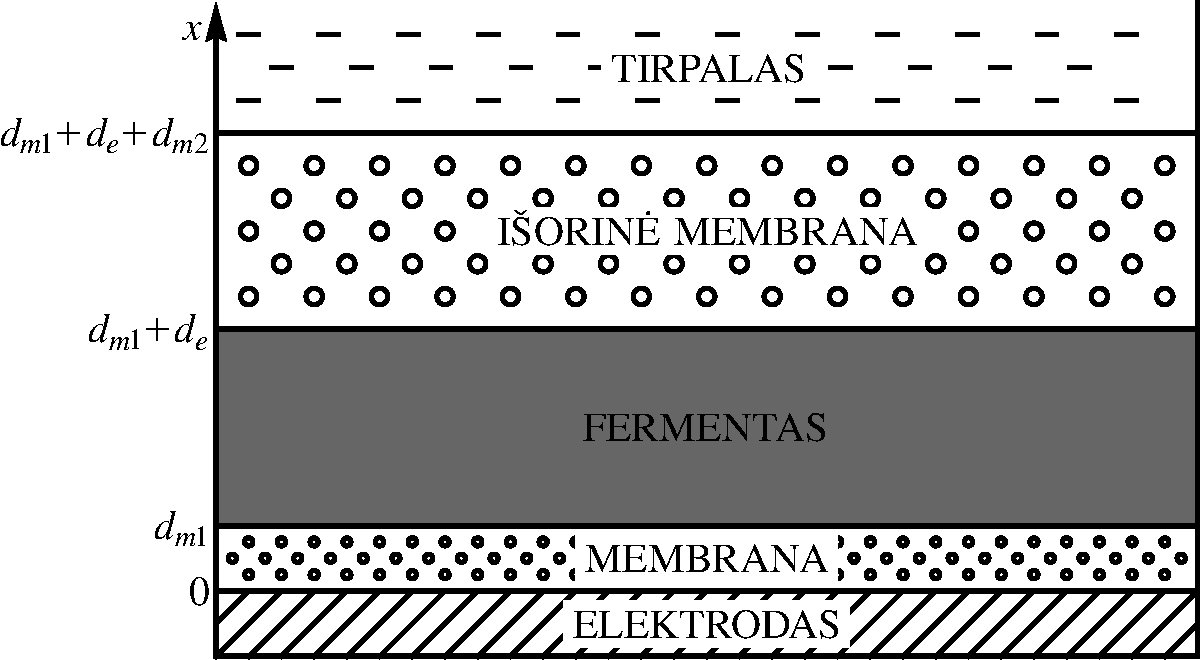
\includegraphics[clip=true, width=0.65\textwidth]{figures/fig01.pdf}
    \caption{Elektrocheminio biojutiklio sandaros schema. Rodykle pažymėta kintamojo $x$ ašis.}
    \label{pav01}
\end{figure}

Išorinė membrana dažniausiai būna pagaminta iš polimerinio pluošto.
Labai dažnai tai būna celofano plėvelės.
Kartais naudojamos tankios polimerinės plėvelės, kuriose dirbtinai padaryta skylių.
Pavyzdžiui, argono branduoliais prašaudyta teflono plėvelė -- po elektroniniu mikroskopu tokia plėvelė atrodo kaip medžioklinio šautuvo šratais sušaudytas faneros lakštas.

\subsubsection{Antras iliustracijos pavyzdys}

Kraštinės sąlygos substrato koncentracijai $S$ modeliavimo srities $0 \leqslant x \leqslant d_{m1} + d_e + d_{m2}$ kraštuose formuluojamos
atsižvelgiant į tai, kad į elektrodą substratas įsiskverbti negali, o tirpale (į kurį panardintas biojutiklis) yra palaikoma pastovi substrato koncentracija $S_0$:
\begin{equation}
    \left. \frac{\partial S}{\partial x} \right|_{x=0}  =  0,  \qquad
    S( x = d_{m1} + d_e + d_{m2}, t )  =  S_0,  \qquad  t > 0.
    \label{KrastinesSalygosSAtzvilgiu}
\end{equation}

Be to, darome prielaidą, kad ant elektrodo produktas labai greitai reaguoja.
Todėl produkto koncentracija $P( x = 0 ,t )$ (ant briaunos su elektrodu) visą laiką bus lygi nuliui.

Modeliuodami nagrinėsime du skirtingus atvejus.

\medskip
\textbf{Difunduojančio į tirpalą produkto atvejis.}
Tarkime, išorinės membranos sienelė leidžia produktui difunduoti į tirpalą.
Tuomet produkto koncentracija $P$ intervalo $0 \leqslant x \leqslant d_{m1} + d_e + d_{m2}$ kraštuose tenkina sąlygas
\begin{equation}
    P( x = 0, t )  =  0,  \qquad
    P( x = d_{m1} + d_e + d_{m2}, t )  =  0,  \qquad  t > 0.
    \label{KrastinesSalygosPAtzvilgiu}
\end{equation}

\medskip
\textbf{Atvejis kai produktas negali patekti į tirpalą.}
Jeigu išorinės membranos sienelė nepralaidi produktui, kraštinėse sąlygose (\ref{KrastinesSalygosPAtzvilgiu}) antroji sąlyga turi būti pakeista reikalavimu,
kad srities krašte funkcijos išvestinė turi būti lygi nuliui (nėra produkto ištekėjimo).
Taigi, tokiu atveju produkto koncentracijai $P$ formuluojame tokias kraštines sąlygas:
\begin{equation}
    P( x = 0, t )  =  0,  \qquad
    \left. \frac{\partial P}{\partial x} \right|_{x=d_{m1}+d_e+d_{m2}}  =  0,  \qquad  t > 0.
    \label{AlternatyviosKrastinesSalygosPAtzvilgiu}
\end{equation}

Jeigu $C_1>0$ ir$/$arba $C_2>0$, tai dėl degradacijos biojutiklio atsakas (nusistovėjęs laike srovės tankis) $I$ sumažėja
(palyginus su atveju be degradacijos $C_1 ={}$\SI{0}{\per\second}, $C_2 ={}$\SI{0}{\per\second}).
Ištirsime šio sumažėjimo priklausomybę nuo parametrų $C_1$ ir $C_2$.

Iliustracijoje \ref{pav02}~pav.\ grafiškai išskirtos parametrų erdvės $\left( C_1, C_2 \right)$ dalys, kurioje biojutiklio atsakas
sumažėja nuo $0$\% iki $1$\% (balta sritis), nuo $1$\% iki $2$\% (balta užbrūkšniuota sritis), nuo $2$\% iki $3$\% (šviesiai pilka sritis), nuo $3$\% iki $4$\% (šviesiai pilka užbrūkšniuota sritis), ir taip toliau -- vis tamsėjant srities fonui.

\begin{figure}[ht!]
    \centering
    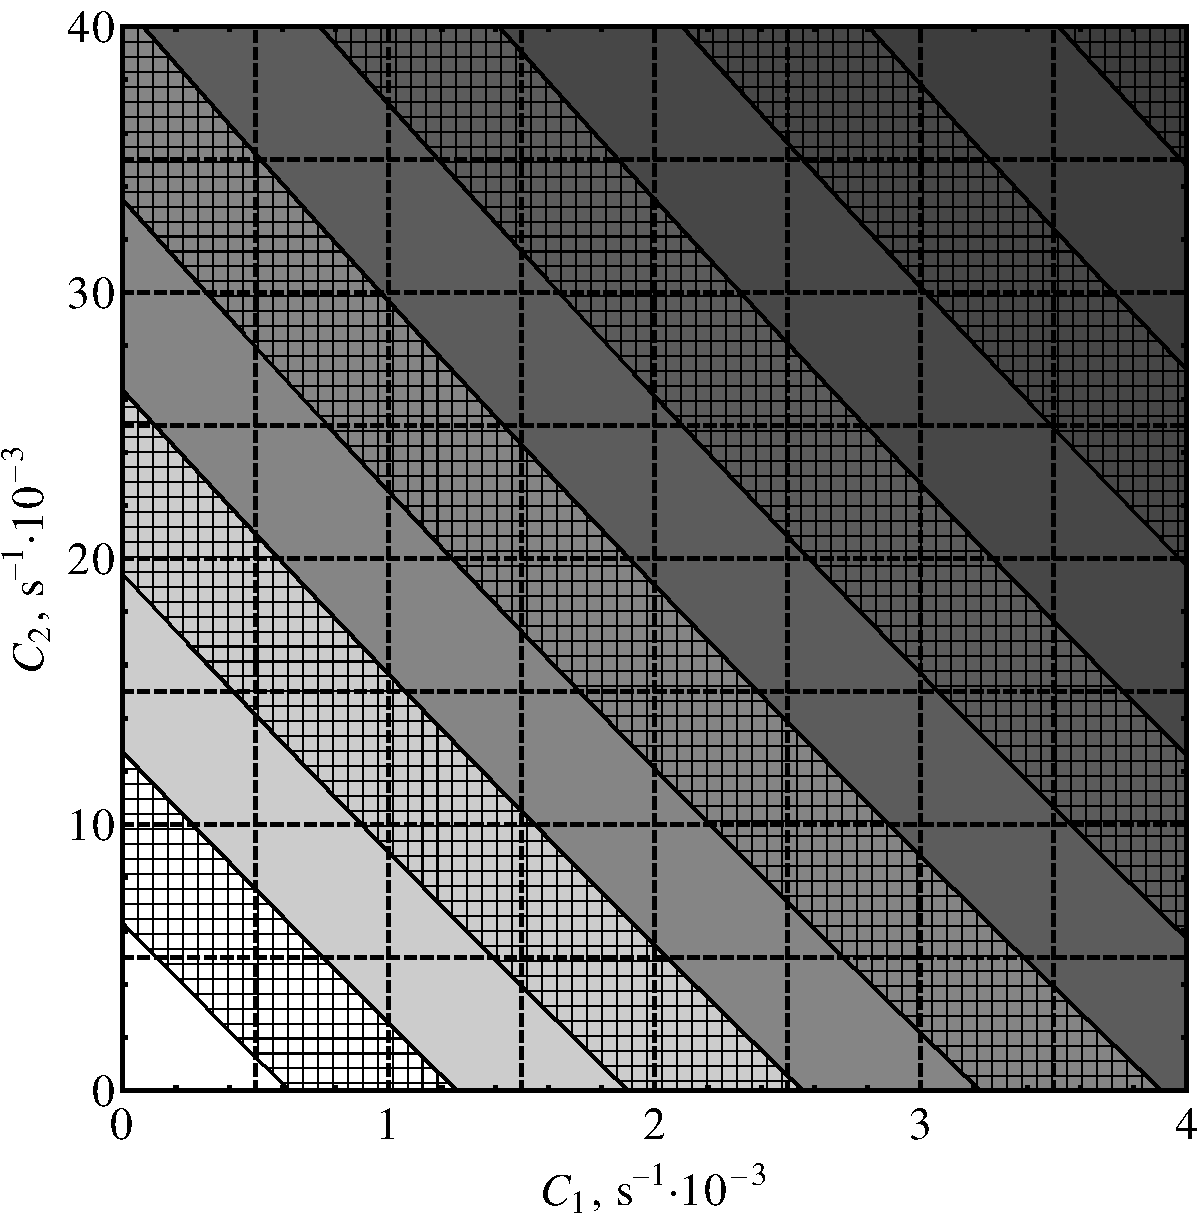
\includegraphics[clip=true, width=0.49\textwidth]{figures/fig02a.pdf}\,
    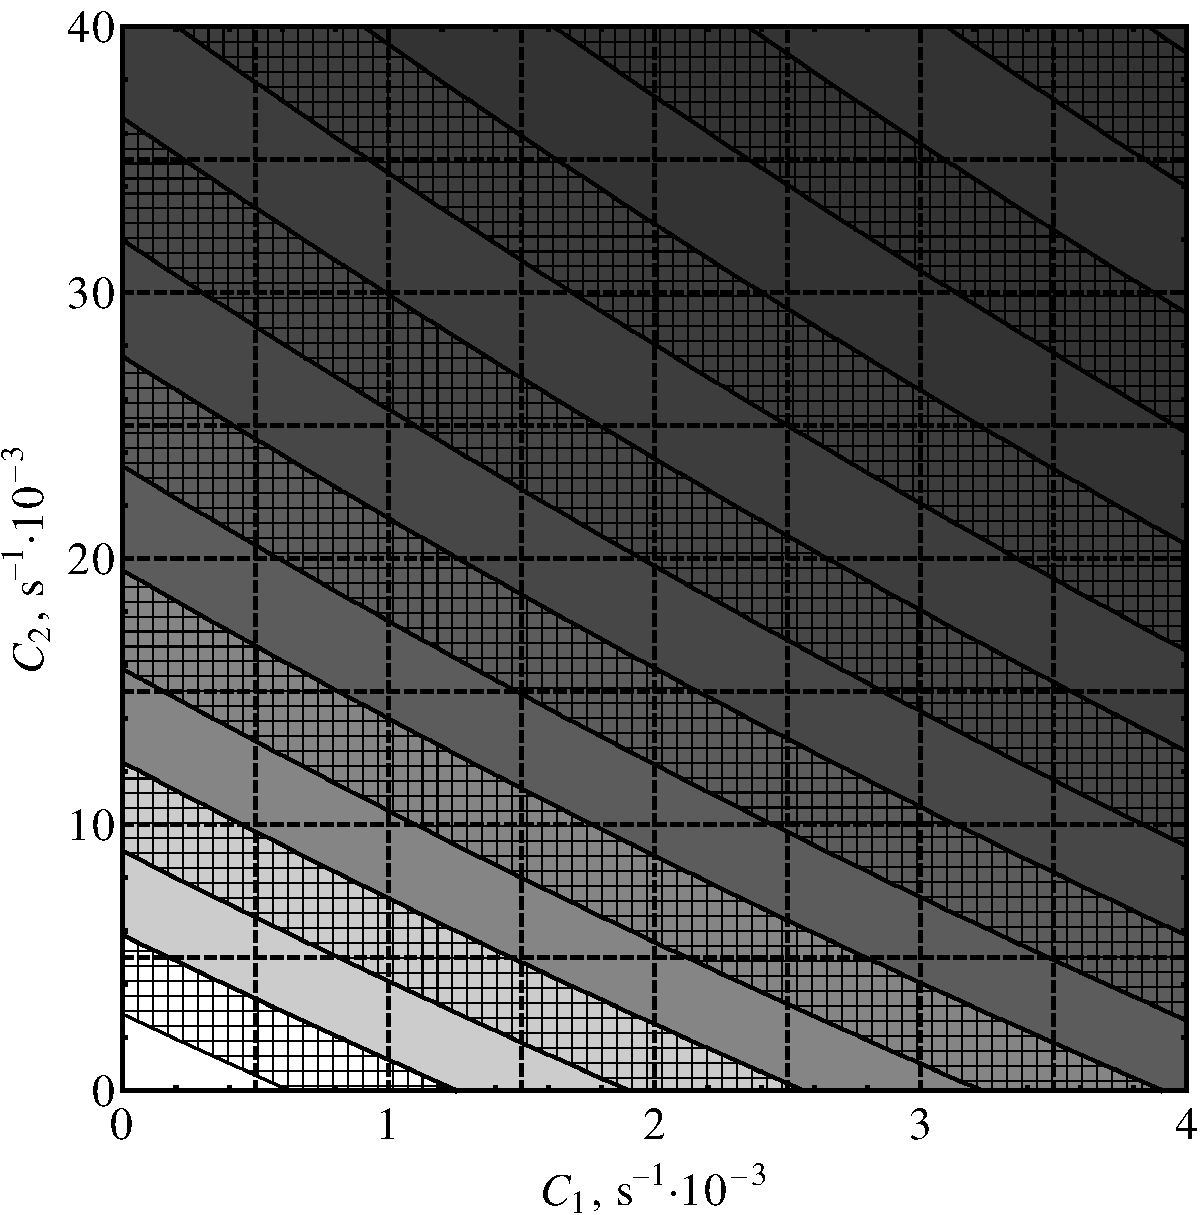
\includegraphics[clip=true, width=0.49\textwidth]{figures/fig02b.pdf}
    \caption{Biojutiklio atsako $I$ degradacija (sumažėjimas) koordinačių ploštumoje $\left( C_1, C_2 \right)$.
    Iliustracija kairėje: kraštinės sąlygos (\ref{KrastinesSalygosPAtzvilgiu}) (difunduojančio į tirpalą produkto atvejis).
    Iliustracija dešinėje: kraštinės sąlygos (\ref{AlternatyviosKrastinesSalygosPAtzvilgiu}) (atvejis kai produktas negali patekti i tirpalą).
    Modelio ir algoritmo parametrai: $N = 100$, $\tau ={}$\SI{0.01}{\second},
    $d_{m1} ={}$\SI{2}{\micro\metre}, $d_e ={}$\SI{9}{\micro\metre}, $d_{m2} ={}$\SI{10}{\micro\metre},
    $D_{S_{m1}} ={}$\SI{6}{\micro\metre\squared\per\second}, $D_{P_{m1}} ={}$\SI{5}{\micro\metre\squared\per\second}, $D_{S_e} ={}$\SI{22}{\micro\metre\squared\per\second},
    $D_{P_e} ={}$\SI{20}{\micro\metre\squared\per\second}, $D_{S_{m2}} ={}$\SI{7}{\micro\metre\squared\per\second}, $D_{P_{m2}} ={}$\SI{6}{\micro\metre\squared\per\second},
    $V_{max} ={}$\SI{0.3}{\milli\mole\per\metre\cubed\per\second},
    $K_M ={}$\SI{0.23}{\mole\per\metre\cubed}, $S_0 ={}$\SI{0.07}{\mole\per\metre\cubed}.}
    \label{pav02}
\end{figure}

Matome, kad skaičiuojant su \ref{pav02}~pav.\ nurodytais parametrais rezultatai gana
\emph{ženkliai priklauso nuo to su kuriomis kraštinėmis sąlygomis apibrėžtas matematinis modelis}:
kraštinėmis sąlygomis (\ref{KrastinesSalygosPAtzvilgiu}) ar (\ref{AlternatyviosKrastinesSalygosPAtzvilgiu}).

Taip pat pastebėkime (žr.\ \ref{pav02}~pav.), kad aiškinantis kokios (skirtingos) parametrų $C_1>0$ ir $C_2>0$ vertės gali sąlygoti kažkokį vieną ir tą patį (fiksuotą) $I$ sumažėjimą,
gaunamas \textit{beveik tiesinis} ryšys tarp parametrų $C_1$ ir $C_2$. Tiesa, iliustracijoje matomos $I$ (vienodo) sumažėjimo izolinijos nėra absoliučiai idealios tiesės.

Verta pastebėti ir tai, kad parametro $C_1$ \textit{įtaka degradacijai keletą kartų didesnė} už parametro $C_2$ įtaką.
Tiesa, kiek būtent kartų -- priklauso ir nuo kraštinių sąlygų pasirinkimo.
Skaičiuojant su kraštinėmis sąlygomis (\ref{KrastinesSalygosPAtzvilgiu}), matyti (žr.\ \ref{pav02}~pav.\ iliustraciją kairėje), kad
parametrų pasirinkimai $C_1 ={}$\SI{4}{\milli(s^{-1})}, $C_2 ={}$\SI{0}{\milli(s^{-1})} ir $C_1 ={}$\SI{0}{\milli(s^{-1})}, $C_2 ={}$\SI{40}{\milli(s^{-1})}
sukelia apytiksliai vienodą nusistovėjusio srovės tankio $I$ sumažėjimą, taigi parametro $C_1$ įtaka apie $10$ kartų didesnė už parametro $C_2$ įtaką.
Tačiau kraštinių sąlygų (\ref{AlternatyviosKrastinesSalygosPAtzvilgiu}) pasirinkimas rodo (žr.\ \ref{pav02}~pav.\ iliustraciją dešinėje), kad
$C_1$ įtaka tik apie $5$ kartus didesnė už $C_2$ įtaką.

\subsubsection{Trečias iliustracijos pavyzdys}

\begin{figure}[ht!]
    \centering
    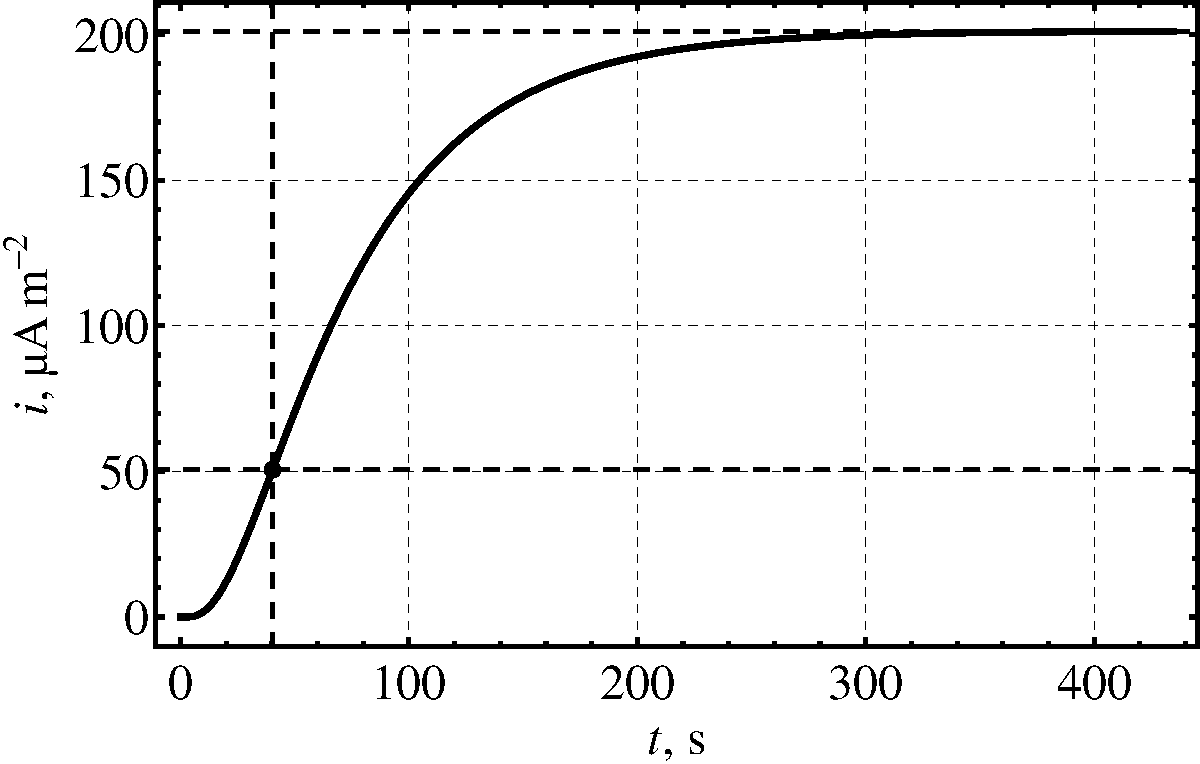
\includegraphics[clip=true, width=0.49\textwidth]{figures/fig03a.pdf}\,
    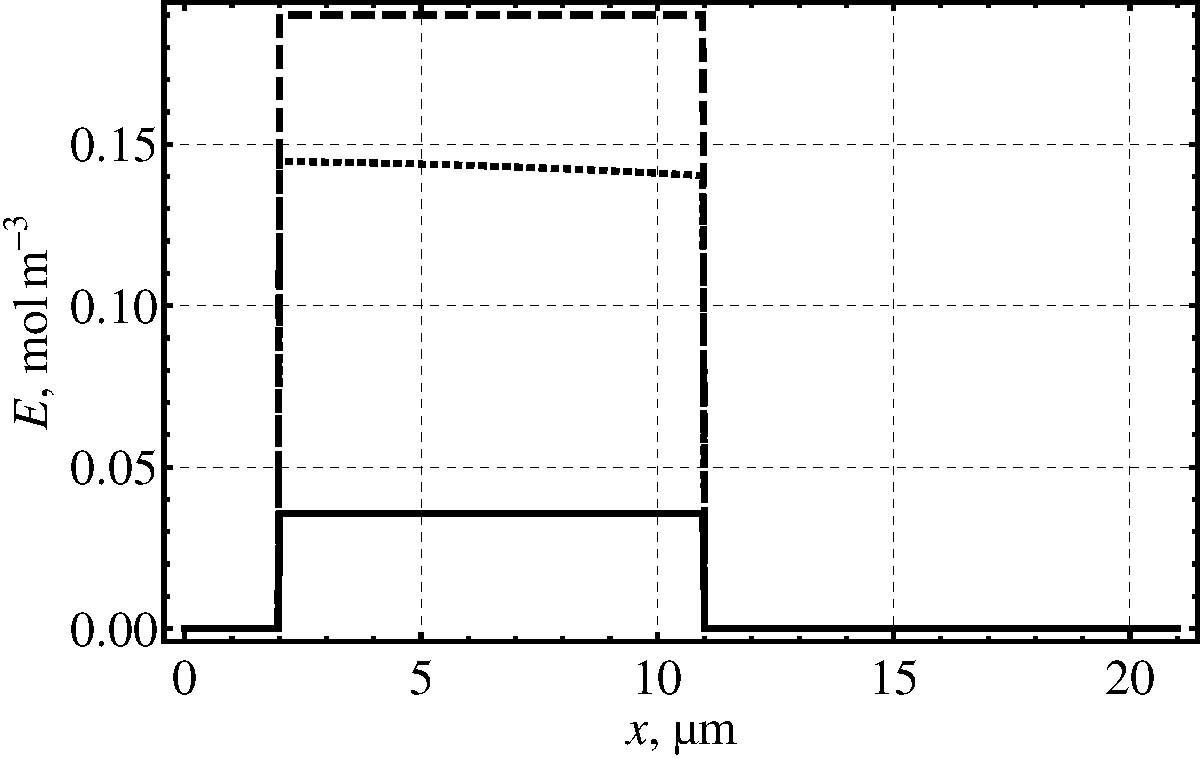
\includegraphics[clip=true, width=0.49\textwidth]{figures/fig03b.pdf}
    \caption{Iliustracija kairėje: srovės tankio $i(t)$ priklausomybė nuo laiko $t$ (punktyru paryškinti laiko momentas $t = t_{slopeMAX}$ ir biojutiklio atsakas $I$).
    Iliustracija dešinėje: fermento koncentracijos $E(x,t)$ priklausomybės nuo biojutiklio koordinatės $x$,
    laiko momentu $t ={}$\SI{1}{\second} (brūkšninė kreivė),
    laiko momentu $t = t_{slopeMAX}$ (taškinė kreivė) ir
    laiko momentu $t = t_I$ (ištisinė kreivė).}
    \label{pav03ab}
    \bigskip
    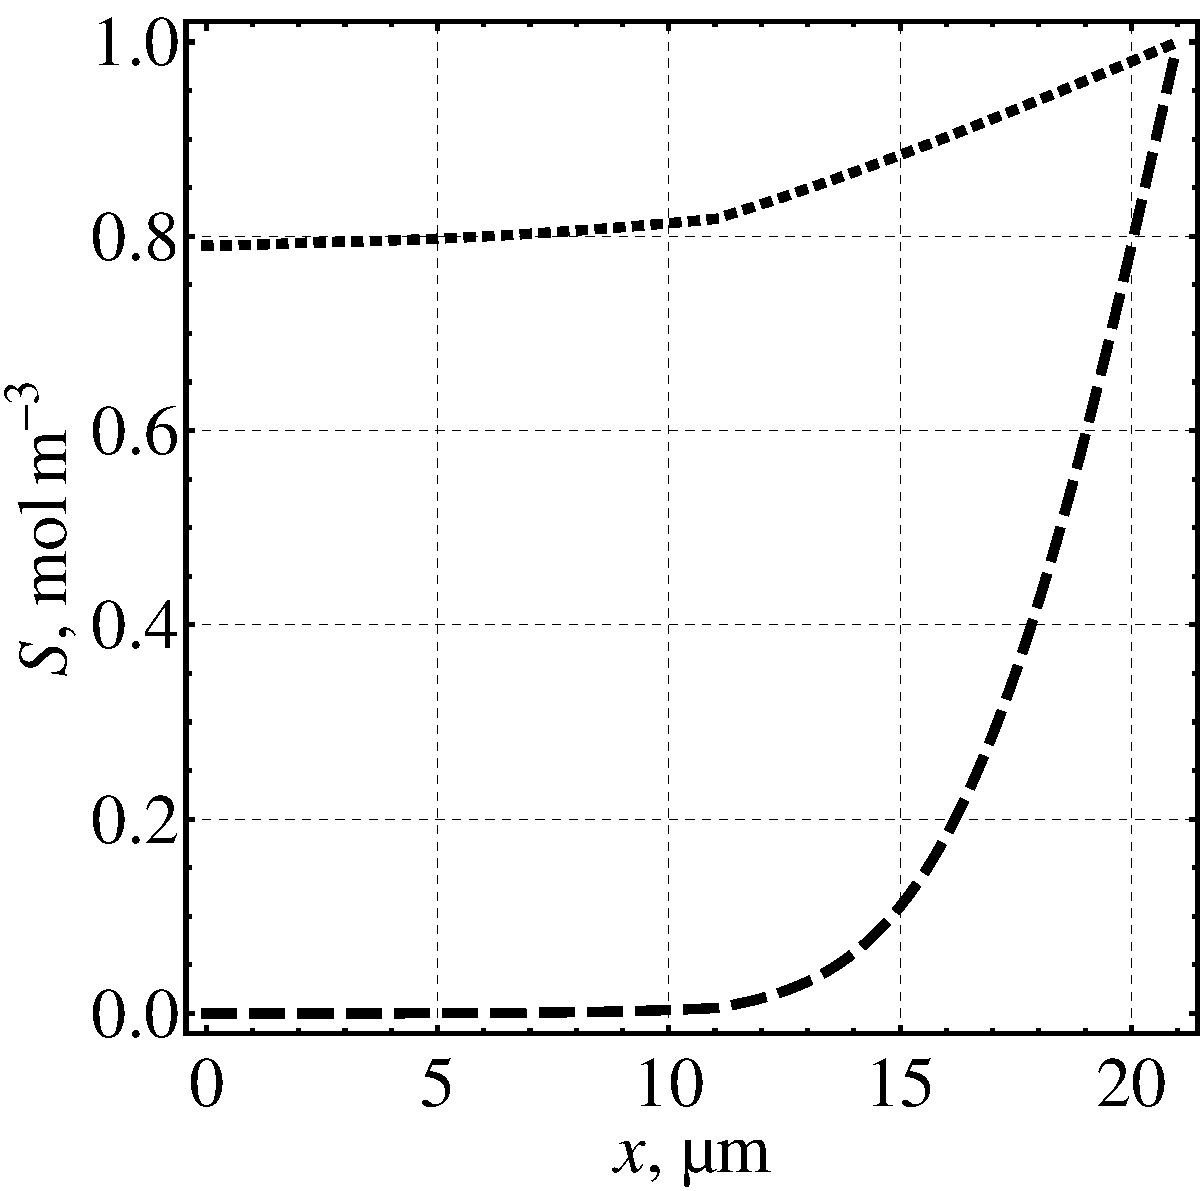
\includegraphics[clip=true, width=0.32\textwidth]{figures/fig03c.pdf}\,
    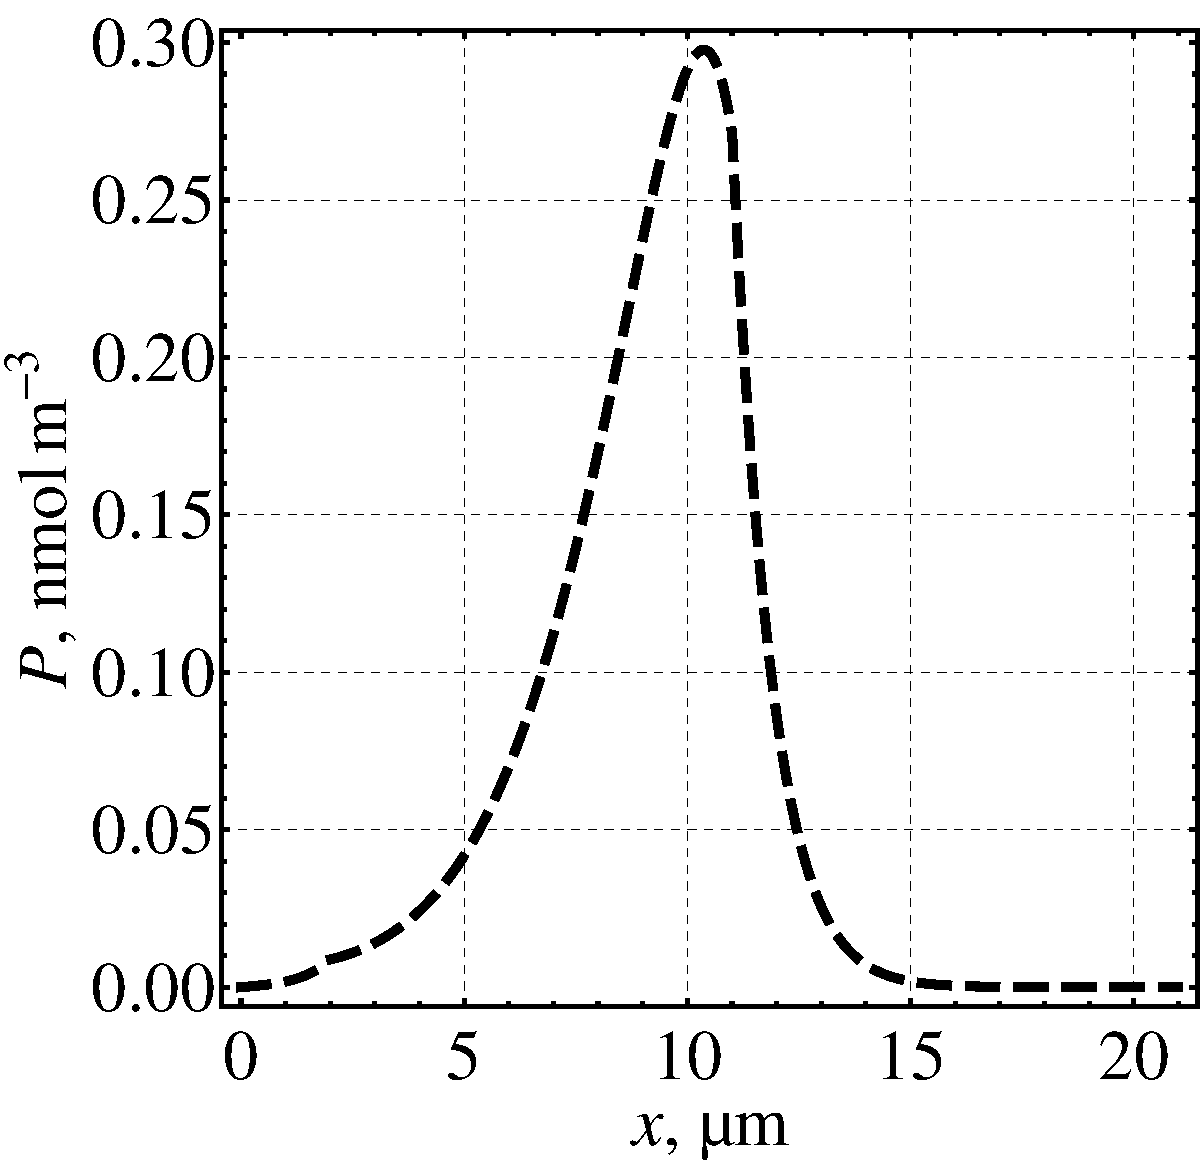
\includegraphics[clip=true, width=0.33\textwidth]{figures/fig03d.pdf}\,
    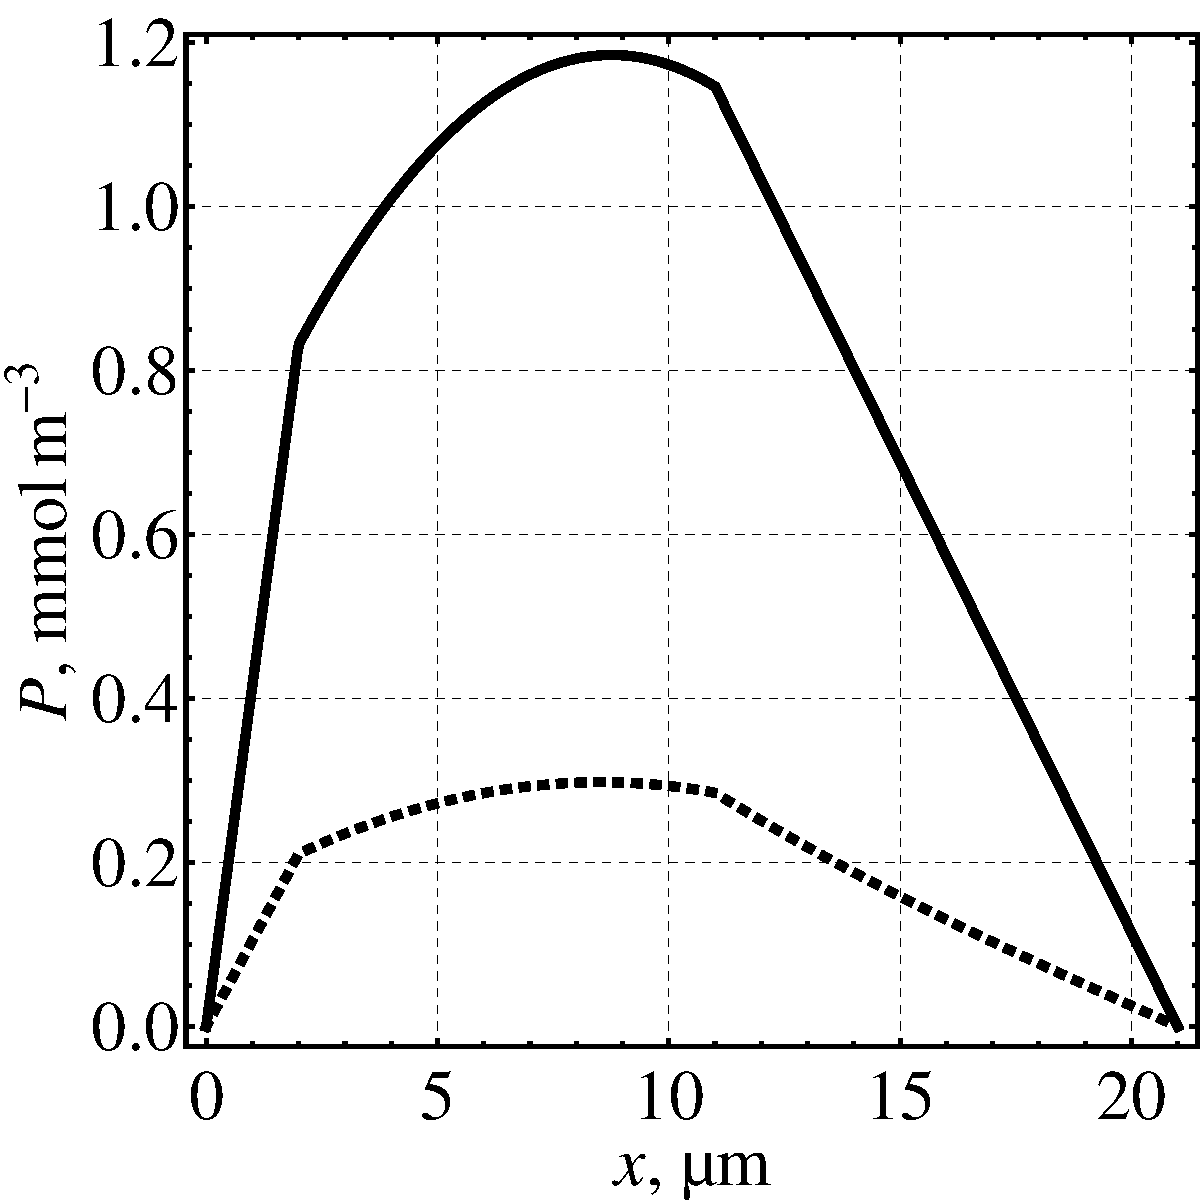
\includegraphics[clip=true, width=0.32\textwidth]{figures/fig03e.pdf}
    \caption{Iliustracija kairėje: substrato koncentracijos $S(x,t)$ priklausomybės nuo biojutiklio koordinatės $x$,
    laiko momentu $t ={}$\SI{1}{\second} (brūkšninė kreivė) ir
    laiko momentu $t = t_{slopeMAX}$ (taškinė kreivė).
    Iliustracija centre: produkto koncentracijos $P(x,t)$ priklausomybė nuo biojutiklio koordinatės $x$,
    laiko momentu $t ={}$\SI{1}{\second} (brūkšninė kreivė).
    Iliustracija dešinėje: produkto koncentracijos $P(x,t)$ priklausomybės nuo biojutiklio koordinatės $x$,
    laiko momentu $t = t_{slopeMAX}$ (taškinė kreivė) ir
    laiko momentu $t = t_I$ (ištisinė kreivė).}
    \label{pav03cde}
\end{figure}

Skaičiavimai vykdyti su matematinio modelio ir algoritmo parametrais:
kraštinės sąlygos (\ref{KrastinesSalygosPAtzvilgiu}) (difunduojančio į tirpalą produkto atvejis),
$N = 1000$, $h ={}$\SI{0.021}{\micro\metre}, $\tau_{max} ={}$\SI{0.01}{\second},
$d_{m1} ={}$\SI{2}{\micro\metre}, $d_e ={}$\SI{9}{\micro\metre}, $d_{m2} ={}$\SI{10}{\micro\metre},
$C_1 ={}$\SI{0}{\per\second}, $C_2 ={}$\SI{0}{\per\second}, $S_0 ={}$\SI{1}{\mole\per\metre\cubed}, $E_0 ={}$\SI{0.19}{\mole\per\metre\cubed},
$k_{+1} ={}$\SI{0.015}{\metre\cubed\per\mole\per\second}, $k_{-1} ={}$\SI{0.0015}{\per\second},
$k_{+3} ={}$\SI{0.002}{\per\second}, $k_{-3} ={}$\SI{0.002}{\metre\cubed\per\mole\per\second}, $n_e = 1$.

\ref{pav03ab}~pav.\ ir \ref{pav03cde}~pav.\ pateikiami rezultatai, kai difuzijos koeficientai yra lygūs:
$D_{S_{m1}} ={}$\SI{6}{\micro\metre\squared\per\second}, $D_{P_{m1}} ={}$\SI{5}{\micro\metre\squared\per\second}, $D_{S_e} ={}$\SI{22}{\micro\metre\squared\per\second},
$D_{P_e} ={}$\SI{20}{\micro\metre\squared\per\second}, $D_{S_{m2}} ={}$\SI{7}{\micro\metre\squared\per\second}, $D_{P_{m2}} ={}$\SI{6}{\micro\metre\squared\per\second}.

Įvertinta biojutiklio atsako reikšmė $I ={}$\SI{201.1}{\micro\ampere\per\metre\squared}, pasiekus laiko momentą $t_I ={}$\SI{434.6}{\second}.
Srovės tankis intensyviausiai augo laiko momentu $t_{slopeMAX} ={}$\SI{40.3}{\second}.

\subsubsection{Ketvirtas iliustracijos pavyzdys}

Ištirsime biojutiklio atsako $I$ penkių procentų degradacijos \emph{izoliniją} (vienodo $I$ santykinio sumažėjimo kreivę) koordinačių plokštumoje $\left( C_1, C_2 \right)$.
Izolinijai priklausantys taškai nusako tokias parametrų $C_1$ ir $C_2$ vertes, su kuriomis nusistovėjęs srovės tankis $I$ sumažėja tiksliai $5$\%
(palyginus su $I$ reikšme, gaunama atveju be degradacijos $C_1 ={}$\SI{0}{\per\second}, $C_2 ={}$\SI{0}{\per\second}).

\begin{figure}[ht!]
    \centering
    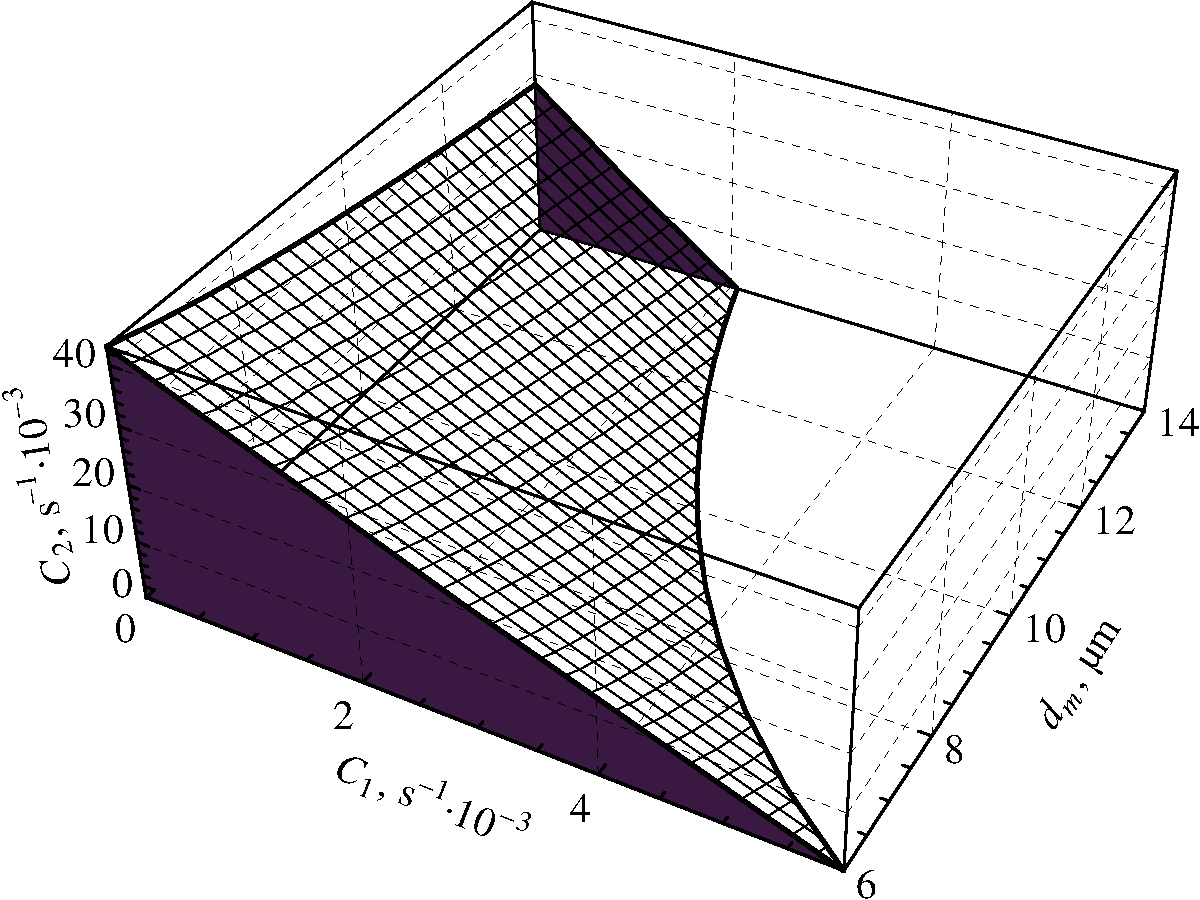
\includegraphics[clip=true, width=0.7\textwidth]{figures/fig04.pdf}
    \caption{Biojutiklio atsako $I$ penkių procentų degradacijos izolinijos (apibrėžtos koordinačių ploštumoje $\left( C_1, C_2 \right)$) priklausomybė (paviršius)
    nuo membranos storio $d_m$.
    Modelio ir algoritmo parametrai:
    $N = 100$, $\tau ={}$\SI{0.01}{\second},
    $d_e ={}$\SI{9}{\micro\metre}, $D_{S_e} ={}$\SI{22}{\micro\metre\squared\per\second}, $D_{P_e} ={}$\SI{20}{\micro\metre\squared\per\second},
    $D_{S_m} ={}$\SI{7}{\micro\metre\squared\per\second}, $D_{P_m} ={}$\SI{6}{\micro\metre\squared\per\second}, $V_{max} ={}$\SI{0.3}{\milli\mole\per\metre\cubed\per\second},
    $K_M ={}$\SI{0.23}{\mole\per\metre\cubed}, $S_0 ={}$\SI{0.07}{\mole\per\metre\cubed}.}
    \label{pav04}
\end{figure}

Ši (ir kitos) izolinija matoma \ref{pav02}~pav. Šiame skyrelyje papildomai panagrinėsime minėtos izolinijos (apibrėžtos koordinačių ploštumoje $\left( C_1, C_2 \right)$)
priklausomybę nuo membranos storio $d_m$ intervale $d_m\in [6,14]$ \si{\micro\metre}.

Skaičiavimų rezultatas pavaizduotas \ref{pav04}~pav.
Matyti, kad sritis po izolinija (\ref{pav04}~pav.\ paryškinta pilkos spalvos fonu) mažėja, didinant $d_m$.
Su parametrais $C_1\geqslant 0$, $C_2\geqslant 0$ iš šios srities (esančios po izolinija) $I$ degradacija neviršyja 5\%.
Pastebėkime, kad visiems $d_m\in [6,14]$ \si{\micro\metre} izolinija apytiksliai išlaiko tiesės pavidalą,
tačiau siekiant ją aproksimuoti dar tiksliau reikėtų naudoti parabolinę kreivę.

Užrašysime izolinijos aproksimacijos tiese analitines priklausomybes nuo parametro $d_m$, galiojančias intervale $d_m\in [6,14]$ \si{\micro\metre},
su \ref{pav04}~pav.\ nurodytais matematinio modelio parametrais.
Remdamiesi skaičiavimo rezultatais, pateiktais \ref{pav04}~pav., mažiausių kvadratų (angliškai ``least squares'') metodu išvedame tokias analitines išraiškas:
\begin{gather}
    C_2  =  K\!\left( d_m \right) C_1  +  M\!\left( d_m \right), \qquad C_1 \geqslant 0, \qquad C_2 \geqslant 0,
    \label{TiesineAproksimacijaAtzvilgiu_dm}\\
    K\!\left( d_m \right)  =  -0.791771\, d_m / \si{\micro\metre}  -  2.48837,
    \label{TiesineAproksimacijaAtzvilgiu_dm_K}\\
    M\!\left( d_m \right)  =  \left. \left( -0.583423\, d_m / \si{\micro\metre}  +  28.3346  +  \frac{110.039}{d_m / \si{\micro\metre}} \right) \right/ 1000.
    \label{TiesineAproksimacijaAtzvilgiu_dm_M}
\end{gather}

Kiekvienam $d_m$, izolinija koordinačių ploštumoje $\left( C_1, C_2 \right)$ eina per taškus
\[
    \left( C_1 = 0, C_2 = M\!\left( d_m \right) \right) \si{\per\second}, \qquad
    \left( C_1 = -\frac{M\!\left( d_m \right)}{K\!\left( d_m \right)}, C_2 = 0 \right) \si{\per\second}.
\]

\subsection{Iliustracijos ir lentelės pavyzdys}

Siekiant dar labiau optimizuoti Cooley--Tukey greitosios Furje transformacijos algoritmą, programuojant galima atsisakyti rekursijos,
o duomenis (signalo reikšmes $f_j$) iš karto išdėstyti tokia tvarka, kokia jie būtų sumuojami paskutiniame (giliausiame) rekursijos lygyje.

Taip pat verta iš anksto suskaičiuoti ir laikyti masyvuose nepriklausančias nuo apdorojamo signalo reikšmių $f_j$ kompleksines konstantas $W_m^{k}$,
tik tokiems sveikiesiems $m$ ir $k$, kuriems šių konstantų iš tiesų prireiks skaičiuojant.

Pasiaiškinsime kokia tvarka Cooley--Tukey algoritme apdorojamos signalo reikšmės $f_j$ bei kurie koeficientai $W_m^{k}$ reikalingi.

Algoritmo veikimo principą galima perprasti nagrinėjant nedaug reikšmių turinčių duomenų atvejį.
Tarkime, $N=8=2^3$. Tuomet duomenys (skaitmeninio signalo reikšmės) yra skaičiai
\[
    f = \left( f_0, f_1, f_2, f_3, f_4, f_5, f_6, f_7 \right).
\]

Mūsų tikslas -- apskaičiuoti dydžius
\begin{gather*}
    C_k = f_0  +  f_1\, W_8^{k}  +  f_2\, W_8^{2k}  +  f_3\, W_8^{3k}  +  f_4\, W_8^{4k}  +  f_5\, W_8^{5k}  +  f_6\, W_8^{6k}  +  f_7\, W_8^{7k}, \\
    k = 0, 1, 2, 3, 4, 5, 6, 7.
\end{gather*}

%%%%%%%%%%%%%%%%%%%%%%%%%%%%%%%%%%%%%%%%%%%%%%%%%%%%%%%%%%%%%%%%%%%%%%%%%%%%%%%%
\noindent\hrulefill
%%%%%%%%%%%%%%%%%%%%%%%%%%%%%%%%%%%%%%%%%%%%%%%%%%%%%%%%%%%%%%%%%%%%%%%%%%%%%%%%

\bigskip
Pirmajame Cooley--Tukey algoritmo rekursijos lygyje, kiekvienam fiksuotam $k=0,1,2,3$ gausime dvi sumas $A_k$ ir $B_k$ iš keturių dėmenų:
\begin{gather*}
    C_k = A_k + W_8^k B_k, \qquad C_{k+4} = A_k - W_8^k B_k, \qquad k = 0, 1, 2, 3,\\
    A_k = \biggl[ f_0  +  f_2\, W_4^{k}  +  f_4\, W_4^{2k}  +  f_6\, W_4^{3k} \biggr], \qquad
    B_k = \biggl[ f_1  +  f_3\, W_4^{k}  +  f_5\, W_4^{2k}  +  f_7\, W_4^{3k} \biggr],
\end{gather*}
arba
\[
    C_k =
    \biggl[ f_0  +  f_2\, W_4^{k}  +  f_4\, W_4^{2k}  +  f_6\, W_4^{3k} \biggr]  +  W_8^k
    \biggl[ f_1  +  f_3\, W_4^{k}  +  f_5\, W_4^{2k}  +  f_7\, W_4^{3k} \biggr].
\]

%%%%%%%%%%%%%%%%%%%%%%%%%%%%%%%%%%%%%%%%%%%%%%%%%%%%%%%%%%%%%%%%%%%%%%%%%%%%%%%%
\noindent\hrulefill
%%%%%%%%%%%%%%%%%%%%%%%%%%%%%%%%%%%%%%%%%%%%%%%%%%%%%%%%%%%%%%%%%%%%%%%%%%%%%%%%

\bigskip
Antrajame rekursijos lygyje kiekvienam fiksuotam $k=0,1$ turėsime jau keturias sumas $AA_k$, $AB_k$, $BA_k$, $BB_k$, kiekvieną iš dviejų dėmenų:
\begin{gather*}
    A_k = AA_k + W_4^k AB_k, \qquad A_{k+2} = AA_k - W_4^k AB_k,\\
    B_k = BA_k + W_4^k BB_k, \qquad B_{k+2} = BA_k - W_4^k BB_k, \qquad k = 0, 1,\\
    AA_k = \Bigl( f_0  +  f_4\, W_2^{k} \Bigr), \qquad
    AB_k = \Bigl( f_2  +  f_6\, W_2^{k} \Bigr),\\
    BA_k = \Bigl( f_1  +  f_5\, W_2^{k} \Bigr), \qquad
    BB_k = \Bigl( f_3  +  f_7\, W_2^{k} \Bigr),
\end{gather*}
arba
\[
    C_k =
    \biggl[  \Bigl( f_0  +  f_4\, W_2^{k} \Bigr)  +  W_4^{k} \Bigl( f_2  +  f_6\, W_2^{k} \Bigr) \biggr]  +  W_8^k
    \biggl[ \Bigl( f_1  +  f_5\, W_2^{k} \Bigr)  +  W_4^{k} \Bigl( f_3  +  f_7\, W_2^{k} \Bigr) \biggr].
\]
%%%%%%%%%%%%%%%%%%%%%%%%%%%%%%%%%%%%%%%%%%%%%%%%%%%%%%%%%%%%%%%%%%%%%%%%%%%%%%%%
\noindent\hrulefill
%%%%%%%%%%%%%%%%%%%%%%%%%%%%%%%%%%%%%%%%%%%%%%%%%%%%%%%%%%%%%%%%%%%%%%%%%%%%%%%%

\bigskip
Trečiajame rekursijos lygyje formaliai būtų apibrėžtos aštuonios ``sumos'', kiekviena sudaryta iš vienintelio dėmens -- signalo reikšmės.
Kokia tvarka išsidėsčiusios šios reikšmės ir iš kokių koeficientų juos reikės padauginti sumuojant, matyti jau iš antrojo rekursijos lygio formulių.
Todėl iš karto galime pereiti prie $1$-ojo algoritmo etapo, kuriame prasideda realūs skaičiavimai.


\begin{figure}[ht!]
    \centering
    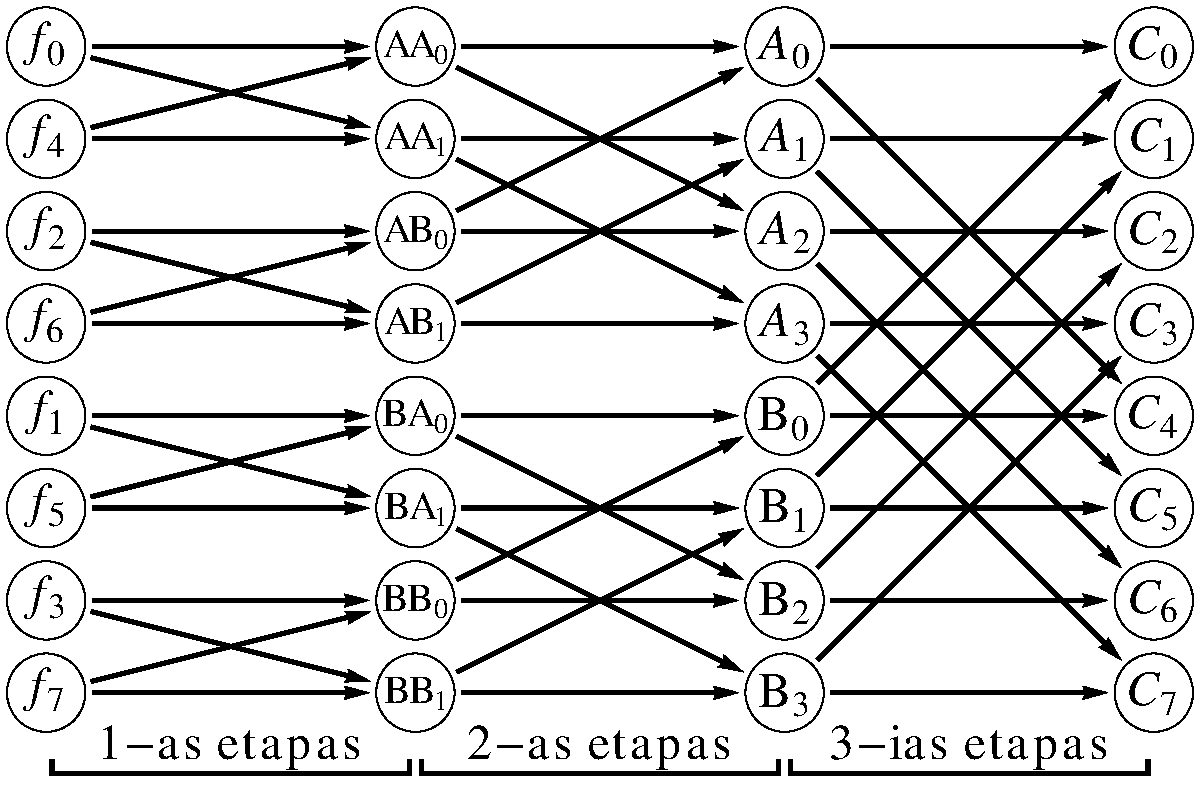
\includegraphics[clip=true, width=0.85\textwidth]{figures/fig05.pdf}
    \caption{Cooley--Tukey greitosios Furje transformacijos algoritme vykdomų aritmetinių operacijų schema $8$ taškų ($N=8$) atveju.
    Rodyklės rodo kurie dydžiai iš praeito algoritmo etapo dalyvauja skaičiuojant sekančio etapo dydžius.}
    \label{pav05}
\end{figure}

\emph{$1$-as etapas}. Naudodami signalo reikšmes $f_j$ ir koeficientus $W_2^k$, $k=0,1$, apskaičiuojame tarpinius dydžius $AA_k$, $AB_k$, $BA_k$, $BB_k$, $k=0,1$.
Skaičiavimo schema pateikta \ref{pav05}~pav. Šioje schemoje rodyklės rodo kurie dydžiai dalyvauja atliekant aritmetines operacijas. Pavyzdžiui,
\[
    AA_0 = f_0  +  f_4\, W_2^{0},
\]
taigi iš $f_0$ ir iš $f_4$ eina po rodyklę į $AA_0$. Rodyklė taip pat reiškia vieną aritmetinę operaciją: $f_4$ dauginamas iš konstantos $W_2^{0}$; rezultatas sudedamas su $f_0$.

Beje, 1-ajame etape prireikia tik vienos konstantos $W_2^{0}=1$ (kadangi $W_2^{1}=-W_2^{0}=-1$).
Kadangi visi daugikliai lygūs vienetui, šiame etape sandaugų skaičiavimo galima išvengti.

\begin{table}[h!]
    \caption{Cooley--Tukey algoritmo optimalaus duomenų $f_j$ išdėstymo tvarka pagal indeksus $j$ su atvirkščiai užrašytais dvejetainiais bitais $8$ taškų ($N=8$) atveju.}
    \label{LenteleAtvirkstineDvejetaine}
    \centering
    \begin{tabular}{>{\centering}p{35mm}>{\centering}p{35mm}>{\centering}p{35mm}>{\centering}p{35mm}}
        \noalign{\bigskip}\hline\noalign{\smallskip}
        Indeksai $j$ tradicine tvarka &
        Dvejetainiai indekso $j$ bitai &
        Indekso $j$ bitai atvirkščiai &
        Indeksai $j$ atvirkščių bitų tvarka
        \tabularnewline
        \noalign{\smallskip}\hline\noalign{\smallskip}
        0  & 000 & 000 & 0
        \tabularnewline
        1  & 001 & 100 & 4
        \tabularnewline
        2  & 010 & 010 & 2
        \tabularnewline
        3  & 011 & 110 & 6
        \tabularnewline
        4  & 100 & 001 & 1
        \tabularnewline
        5  & 101 & 101 & 5
        \tabularnewline
        6  & 110 & 011 & 3
        \tabularnewline
        7  & 111 & 111 & 7
        \tabularnewline
        \noalign{\smallskip}\hline
    \end{tabular}
\end{table}

Taip pat, matome kokia tvarka reikėtų išdėstyti duomenis, kad jie būtų greičiausiai pasiekiami:
\[
    f_0, f_4, f_2, f_6, f_1, f_5, f_3, f_7.
\]

Žiūrint į šią išdėstymo tvarką, sunkoka suvokti kaip ją būtų galima apibendrinti kai $N=16$, $N=32$ ir taip toliau.
Viskas paaiškėja duomenų indeksus išreiškus ne dešimtainėje, bet dvejetainėje skaičiavimo sistemoje, žr.\ \ref{LenteleAtvirkstineDvejetaine}~lentelę.
Tereikia reikšmių $f_j$ indeksų dvejetainius bitus užrašyti atvirkštine (veidrodine) tvarka.

\emph{$2$-as etapas}. Dabar jau naudojame praeitame -- $1$-ajame etape apskaičiuotus dydžius $AA_k$, $AB_k$, $BA_k$, $BB_k$, $k=0,1$ ir
suskaičiuojame šio etapo tarpinius dydžius $A_k$, $B_k$, $k=0,1,2,3$. Skaičiavimo schema matoma \ref{pav05}~pav.

2-ajame etape reikalingos dvi konstantos $W_4^{k}$, $k=0,1$.

\emph{$3$-ias etapas}. Turėdami praeitame ($2$-ajame) etape apskaičiuotus dydžius $A_k$, $B_k$, $k=0,1,2,3$, randame koeficientus $C_k$, $k=0,1,2,3,4,5,6,7$.
Skaičiavimo schema pateikta \ref{pav05}~pav.

3-iajame etape naudojame konstantas $W_8^{k}$, $k=0,1,2,3$.

3-iasis etapas yra paskutinis, kadangi turėjome apdoroti $N=2^3$ ilgio duomenų seką.

Visose algoritmo sandaugose vienas iš dauginamųjų yra kompleksinė konstanta $W_m^{k}$.
Naudojamos tik konstantos (šiems indeksams $m$ ir $k$):
\[
    W_m^k = e^{\displaystyle -i \frac{2\pi}{m} k} = \cos \frac{2\pi k}{m} - i\, \sin \frac{2\pi k}{m}, \quad m = 2, 4, 8, 16, \ldots, N, \quad k =0, 1, \ldots, \frac{m}{2}-1.
\]
Beje, kai $k=0$, $W_m^0=1$.

\medskip\noindent
\textit{Cooley--Tukey algoritmo sudėtingumas}
\nopagebreak
\medskip

Įvertinkime kiek aritmetinių operacijų iš viso daroma Cooley--Tukey algoritme. Atimtį ir sudėtį laikysime ekvivalenčiomis kompiuterio procesoriaus laiko požiūriu operacijomis,
o sandaugas suskaičiuosime atskirai.

Kaip matome iš nagrinėto pavyzdžio, reikalingi $n=\log_2 N$ etapai.
Kiekviename etape skaičiuojama $N$ sudėčių ir $N/2$ sandaugų.
Sandaugų yra dvigubai mažiau nei sudėčių, nes kiekviename etape antroji pusė dydžių skaičiuojama analogiškai kaip pirmoji pusė, tik pakeitus sudėtį į atimtį.
Pavyzdžiui, mūsų nagrinėtame pavyzdyje su $N=8$, $2$-ajame etape skaičiavome dydžius $A_k$ pagal formules
\[
    A_k = AA_k + W_4^k AB_k, \qquad A_{k+2} = AA_k - W_4^k AB_k, \qquad k = 0, 1,
\]
taigi skaičiuojant $A_{k+2}$ nebereikia skaičiuoti sandaugos $W_4^k AB_k$ (ji jau suskaičiuota, randant $A_k$).

Vadinasi, iš viso reikia atlikti $(N/2) \log_2 N$ kompleksinių sandaugų ir $N \log_2 N$ kompleksinių sudėčių.
Sandaugų kiekį galima dar šiek tiek sumažinti, pasinaudojus tuo, kad $W_m^0=1$ bei kitais specialiais konstantų $W_m^k$ atvejais.
Pavyzdžiui, kaip matėme $1$-ajame algoritmo etape galima aplamai išvengti dauginimo veiksmo.

Taigi, Cooley--Tukey algoritmo sudėtingumas yra $O(N \log_2 N)$.

\subsection{Lentelės pavyzdys}

\ref{Table1}~lentelėje ištirta koks yra defektų tankio $N_{def}$ įverčio santykinis tikslumas.

% \tabcolsep reikšmė kontroliuoja tarpus tarp lentelės stulpelių
\setlength{\tabcolsep}{7pt}
\begin{table}[ht!]
    \caption{Defektų tankio $N_{def}$ įverčių santykinės paklaidos.}
    \label{Table1}
    \centering
    \begin{tabular}{rrrrr}
        \noalign{\bigskip}\hline\noalign{\smallskip}
        \multicolumn{1}{c}{Defekto} &
        \multicolumn{1}{c}{Dažnis} &
        \multicolumn{1}{c}{Tikslus} &
        \multicolumn{1}{c}{Įvertintas} &
        \multicolumn{1}{c}{Santykinė} \\
        \multicolumn{1}{c}{spindulys} &
        \multicolumn{1}{c}{$f_{min}$, \si{\hertz}} &
        \multicolumn{1}{c}{$N_{def}$,} &
        \multicolumn{1}{c}{$N_{def}$,} &
        \multicolumn{1}{c}{paklaida} \\
        \multicolumn{1}{c}{$r_0$, \si{\nano\meter}} & &
        \multicolumn{1}{c}{\si{\per\micro\meter\squared}} &
        \multicolumn{1}{c}{\si{\per\micro\meter\squared}} \\
        \noalign{\smallskip}\hline\noalign{\smallskip}
        $1$    & $516$    & $2.89\cdot 10^1$ & $3.02\cdot 10^1$ & $4.5$\% \\
        $10$   & $1090$   & $2.89\cdot 10^1$ & $3.81\cdot 10^1$ & $32.1$\% \\
        \noalign{\smallskip}\hline\noalign{\smallskip}
        $1$    & $3.3$    & $2.89\cdot 10^{-1}$ & $2.72\cdot 10^{-1}$ & $5.7$\% \\
        $10$   & $5.02$   & $2.89\cdot 10^{-1}$ & $2.57\cdot 10^{-1}$ & $11.0$\% \\
        $100$  & $9.78$   & $2.89\cdot 10^{-1}$ & $3.01\cdot 10^{-1}$ & $4.3$\% \\
        \noalign{\smallskip}\hline\noalign{\smallskip}
        $1$    & $0.0242$ & $2.89\cdot 10^{-3}$ & $2.83\cdot 10^{-3}$ & $2.0$\% \\
        $10$   & $0.0328$ & $2.89\cdot 10^{-3}$ & $2.39\cdot 10^{-3}$ & $17.2$\% \\
        $100$  & $0.0502$ & $2.89\cdot 10^{-3}$ & $2.26\cdot 10^{-3}$ & $21.7$\% \\
        $1000$ & $0.0976$ & $2.89\cdot 10^{-3}$ & $2.62\cdot 10^{-3}$ & $9.3$\% \\
        \noalign{\smallskip}\hline
    \end{tabular}
\end{table}

\subsection{Pseudokodo pavyzdys}
\label{PseudokodoPvz}

Kartais kyla poreikis sugeneruoti tam tikromis statistinėmis savybėmis pasižymintį signalą kompiuteriu. Tokie signalai vadinami \emph{sintetinės kilmės} signalais
arba signalų \emph{simuliacijomis}, kadangi jie nėra jokio realiame gyvenime vykstančio proceso eksperimentiniai duomenys, o tik jų matematinė imitacija.

Sintetinės kilmės signalus galima lengvai ir greitai generuoti, tuo tarpų realių eksperimentinių duomenų surinkimas reikalauja nepalyginamai daugiau laiko ir kitų
išteklių. Tokie sintetiniai signalai gali būti ir yra naudojami akademiniams tikslams, matematinių modelių palyginimui su eksperimentiniais rezultatais,
kompiuterinių algoritmų realizacijų testavimui.
Pavyzdžiui, labai patogu kompiuterinės simuliacijos būdu imituoti įvairius triukšmus, pasižyminčius reikiamomis savybėmis.

Sintetiniai signalai gaunami iš tam tikros matematinės formulės arba išsprendus duotą matematinį modelį (pavyzdžiui, rekurentinius sąryšius, diferencialinę lygtį ir pan.).
Matematinė formulė arba modelis gali būti determinuoti (be atsitiktinai kintančių dydžių). Tokiu atveju tiesiog užprogramuojame šią formulę arba algoritmą duotam
modeliui spręsti.

Tačiau dažnai reikia programuoti signalų simuliacijas, kuriose yra vienas ar daugiau atsitiktinai kintantys dydžiai. Pavyzdžiui, simuliuojant triukšmą,
atsitiktinai klaidžiojančios dalelės judėjimą, miesto transporto atvykimo laikus ir t.\,t.\

Laikysime, kad žinome kaip kompiuteriu gauti pseudoatsitiktinį skaičių su vienoda tikimybe įgyjantį bet kurį intervalo $[0,1)$ tašką (dar vadinamą atsitiktiniu dydžiu,
tolygiai pasiskirsčiusiu intervale $[0,1)$). Tokius skaičius žymėsime $u_1$, $u_2$, ir taip toliau.
Visos programavimo kalbos ir aplinkos turi priemones tokiems skaičiams gauti.

Reikėtų pasakyti, kad dauguma programavimo kalbų ir aplinkų instrumentų šiuos pseudoatsitiktinius skaičius generuoja gana primityviai, todėl jų atsitiktinumas
yra paviršutiniškas. Todėl rimtuose taikymuose reikėtų naudoti specialias programų bibliotekas, taikančias specializuotus algoritmus
(pavyzdžiui, ``Mersenne twister'' metodą) kokybiškų pseudoatsitiktinių skaičių $u_1$, $u_2$, ir t.\,t.\ gavimui.

Puasono atsitiktinis dydis $X \sim P(\lambda)$ arba atsitiktinis dydis iš Puasono pasiskirstymo (angliškai ``Poisson distribution'') su parametru $\lambda$
naudojamas aptarnavimo teorijos modeliuose, pavyzdžiui atsitiktinai generuojant laiką, kurį klientui reikės laukti kirpykloje, poliklinikoje, autobuso stotelėje ir pan.,
kai žinoma statistiškai vidutinė laukimo trukmė $\lambda>0$.
Taigi, parametras $\lambda>0$ nusako Puasono atsitiktinio dydžio vidurkį, taip pat ir dispersiją (šiame pasiskirstyme vidurkis ir dispersija sutampa).
Reikia pažymėti, kad Puasono atsitiktinis dydis įgyja tik natūrines reikšmes.

\emph{Metodas Puasono atsitiktinio dydžio generavimui}.
Tarkime, kad $u_1, u_2, \ldots \in [0,1)$ yra tarpusavyje nepriklausomi, pseudoatsitiktiniai skaičiai, tolygiai pasiskirstę intervale $[0,1)$.
Skaičiuojame sandaugas: $u_1$, $u_1 u_2$, $u_1 u_2 u_3$ ir t.\,t., kol sandauga tampa mažesne už $e^{-\lambda}$.
Tuomet dauginamųjų skaičius $n$ \emph{priešpaskutinėje} sandaugoje kurioje $e^{-\lambda}$ vis dar buvo viršijamas: $u_1 u_2 \cdots u_n \geqslant e^{-\lambda}$
ir yra pseudoatsitiktinis skaičius iš Puasono pasiskirstymo su parametru $\lambda>0$. Šio algoritmo pseudokodas:

\bigskip
\begin{minipage}[v]{0.9\textwidth}
    \begin{algorithmic}
        \STATE $a = e^{-\lambda}$;
        \STATE $r = 1$;
        \STATE $n = -1$;
        \hspace{10mm}\WHILE{ $r > a$ }
            \STATE sugeneruojame pseudoatsitiktinį $u \in [0,1)$;
            \STATE $r = r * u$;
            \STATE $n = n + 1$;
        \ENDWHILE
        \RETURN $n$;
    \end{algorithmic}
\end{minipage}
\bigskip

Atsitiktinių dydžių iš įvairių pasiskirstymų kompiuterinis generavimas taip pat įmanomas naudojantis tam tikslui skirtais kompiuteriniais įrankiais.

 %the main part
\newpage
\section{Šablonas}
\label{sec:template}
Darbų rašymams rekomenduojama naudoti katedros \LaTeX\ šabloną.




\subsection{Darbų tipai}
Kompiuterijos katedros kuruojamų studijų programų studentai studijų
metu turi rašyti skirtingų tipų rašto darbus. Rašto darbo tipas
nurodomas rašto darbo ataskaitos viršelyje. Darbų tipai su vertimais į
anglų kalbą pateikiami \ref{tab:typesRep} lentelėje.

\begin{table}[h!]\centering\small
\caption{Rašto darbų tipai}
\label{tab:typesRep}
\begin{tabular}{|c|c|c|}
\hline
Tipas&Vertimas&Pakopa\\\hline
Kursinis darbas& Semester Project& BSc\\
Problemų sprendimu grįstas projektas&Problem-Based Project&BSc\\ 
Problemų sprendimu grįstas projektas II d.&Problem-Based Project. Part II&BSc\\ 
Bakalauro baigiamasis darbas& Final Bachelor Thesis&BSc\\\hline
Mokslo tiriamasis darbas I/II&Scientific Research I/II&MSc\\
Mokslo tiriamojo darbo projektas&Scientific Research Project&MSc\\
Magistro baigiamasis darbas&Final Master Thesis&MSc\\\hline
\emph{Dalyko ataskaita} &\emph{Subject Related Report}&BSc\\
Objektinis programavimas. Mini-projektas&Object-Oriented Programming. Mini-Project&\\
Objektinis-programavimas. Recenzija&Object-Oriented Programming. Peer-Review&\\
\hline
\end{tabular}
\end{table}

Skirtingi dalykai turi skirtingus rašto darbus, pavyzdžiui,
mini-projektą, recenziją, projekto dokumentaciją, reikalavimų aprašą
ar pan. Taigi dalykų rašto darbų tipai gali būti skirtingi.

Darbai gali būti rašomi lietuvių arba anglų kalba. Šablone įjungiama
speciali žymė nurodo kalbą. Šablone daroma prielaida, kad vieną darbą
gali atlikti iki penkių studentų.

\subsection{Dokumento struktūra}
Rašto darbuose Santrauka (ir Summary), Įvadas, Išvados, Literatūros
šaltiniai, Sutartinių terminų sąrašas yra nenumeruojami, bet vis tiek
turi būti įtraukti į darbo turinį. Šablone yra sukurta komanda \emph{sectionWithoutNumber}, skirta nenumeruojamiems skyriams sukurti kartu su standartine žyme, pavyzdžiui, \emph{sec:intro}.

Kai kuriuose darbuose, pavyzdžiui, projektų ataskaitose, reikalinga
pratarmė, kurioje paaiškinama, kurį semestrą atliktas darbas,
padėkojama už suteiktus duomenis ar pagalbą (skirtą laiką). Padėka
išreiškiama išoriniams žmonėms iš kitų Vilniaus universiteto padalinių
ar įmonių. Patarmėje taip pat galima paaiškinti, kurios darbo dalys
yra iš ankstesnio darbo etapo, jei darbas yra tęstinis. Kai darbą
atlieka studentų grupė, studentų parašai gali būti pratarmės
puslapyje. Šablone yra nustatoma speciali žymė
\emph{signaturesOnTitlePage}, kuri parašo vietas sugeneruoja arba ant
viršelio, arba pratarmės puslapyje.

Dažniausiai santraukoje būna 100--200 žodžių. Žodžiams skaičiuoti
galima panaudoti Unix komandą \emph{wc -w failoVardas} \cite{LinuxCom}.
Šablone santrauka, santrauka anglų kalba, pratarmė, įvadas, išvados
yra atskiruose \LaTeX\ failuose.


\subsection{Literatūros šaltiniai}
Visi literatūros šaltinių sąraše esantys elementai turi būti
referuojami (cituojami) tekste. Naudojant \LaTeX , bibliografinius
šaltinius valdo įrankis \BibTeX. Šaltiniai būna skirtingų
tipų. Pavyzdžiui, \cite{Cormen} ir \cite{Spatial} šaltiniai yra
knygos, \cite{SSJ14} šaltinis yra straipsnis žurnale, o \cite{SJK03}
yra straipsnis konferencijoje. Beje, mokslinių straipsnių, knygų ir
pan. \BibTeX ~šaltinių paruoštukus \emph{bib} formatu galima rasti
kompiuterių mokslo bibliografijoje \emph{dblp} \cite{dblp}.

Rašto darbuose reikia naudoti ir referuoti tik patikimus
šaltinius. Taip pat šaltinių sąraše gali būti duomenų šaltinis,
pavyzdžiui, statistiniai duomenys gali būti imami iš Europos komisijos
duomenų bazės~\cite{Eurostat}. Informatikos terminų vertimus į
lietuvių kalbą galima pasitikslinti Kompiuterinių terminų
žodyne~\cite{KTZ}.

\subsection{Pseudo-kodas ir programinio kodo dalys}

Algoritmus rekomenduojama pateikti pseudo-kodu. Šablone pagal
nutylėjimą yra įtraukti paketai \emph{algorithm} ir
\emph{algorithmic}. Naudojant šiuos paketus pseudo-kode galima turėti
žymes kodo eilutėms. Pavyzdžiui, \ref{lab:alg1}~algoritme
\ref{alg:condition}~eilutė pažymi pseudo-kodo sąlygą. Pagal nutylėjimą
įvesties ir išvesties parametrai žymimi lietuviškais terminais Įvestis
ir Išvestis, bet juos galima pakeisti. Algoritmus galima aprašyti ir
naudojant kitą paketą \emph{algorithm2e}.

\begin{algorithm}
\caption{Algoritmo pavyzdys}
\label{lab:alg1}
\begin{algorithmic}[1]
\REQUIRE $a,b,c\in \mathbb{N}$
\ENSURE $x:\{\mathtt{true,false}\}\times\mathbb{N} $
\IF{$a<b\; \AND\; b<c$}\label{alg:condition}
\STATE $a \leftarrow c$
\RETURN $(\mathtt{false},a)$
\ENDIF
\RETURN $(\mathtt{true},a)$
\end{algorithmic}
\end{algorithm}

Jeigu prireikia nurodyti programų išeities kodo dalis, galima naudotis
\emph{listings} paketu, pavyzdys yra pateiktas \ref{code:first}~
išeities kode. Šiame dokumente įjungta Java programavimo kalba kaip
parametras, nors paketas palaiko nemažą aibę skirtingų paradigmų
kalbų.


\begin{lstlisting}[language=Java,caption={Java metodo pateikimo pavyzdys},label={code:first},emph={0},emphstyle=\color{red}]
boolean method(String a, String b){
  if (a.contains(b)) return true;
  return false;
}
\end{lstlisting}

\subsection{Paveikslėlių paruošimas}
Turint duomenų, tinkamai juos paruošti kaip paveikslėlius (grafikus)
galima tarpplatforminiu įrankiu Gnuplot \cite{GnuPlot}. Pavyzdžiui,
statistinių duomenų blokas, pateiktas \ref{tabl:EUdata}~lentelėje, yra
atvaizduotas \ref{fig:EUplot}~pav, o paveikslėlis buvo sugeneruotas
Gnuplot įrankiu ir panaudojant kodą iš \ref{code:sec}~išeities kodo.



\ref{ex:one} pavyzdyje yra pateikiamas duomenų blokas ir jo pateikimas grafiku, kuris generuojamas Gnuplot įrankiu.


\begin{example}\label{ex:one}
Čia pradedamas pavyzdys. Pavyzdžio pabaigą rodo kvadratėlis. Nors paveikslėliai ir lentelė priklauso pavyzdžiui, jie tekste gali ,,plaukioti.''

\begin{table}[htbp]\caption{Judrūs studentai pagal kilmę~\cite{Eurostat}}
\label{tabl:EUdata}\centering
\begin{tabular}{cccc}
&2010&2011&2012\\\hline
Lietuva&3103 &3129& 3379\\
Latvija&1760&1979&2716\\
Estija&2556&2686&2819\\
\end{tabular}
\end{table}


\begin{lstlisting}[language=Gnuplot,caption={Gnuplot kodo pavyzdys},label={code:sec},emph={0},float=tb,commentstyle=\color{black},xleftmargin=0.1\textwidth]
# saugoti pvz. pavadinimu skriptas.gpi
# vykdyti gnuplot skriptas.gpi

set terminal pdf monochrome
set output 'EUdataLT.pdf'
set style data histogram 
set samples 11
set boxwidth 0.5 
set style fill pattern border
set style histogram cluster gap 1
set yrange [0:4000]

plot  'dataLT.dat' using 2:xtic(1) title columnheader(2), 
    for [i=3:4] '' using i title columnheader(i)
\end{lstlisting}


\begin{figure}[!htbp]\begin{center}
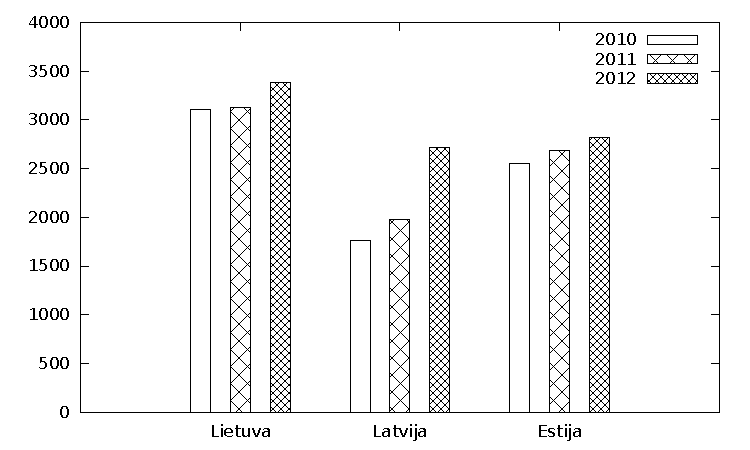
\includegraphics[width=10cm]{figures/EUdataLT}
\end{center}
\caption{Judrių studentų skaičiai. Grafiko y ašyje yra nurodyti studentų skaičiai.}
\label{fig:EUplot}
\end{figure}



\QED
\end{example}

Šablone galima paruošti ir apibrėžimą. Pavyzdžiui, \ref{def:one} apibrėžime apibrėžiamas kelias.

\begin{definition}\label{def:one}
Keliu $k$ laikysime taškų seką $<t_1,...,t_n>$, kai $t_i\in \mathbb{R}\times\mathbb{R}$.
\end{definition}

\subsection{Sudėtingesnės lentelės}
Sudėtingesnėms lentelėms aprašyti gali reikėti papildomų paketų:
ilgoms lentelėms \emph{longtable}, stulpelių/eilučių jungimui
\emph{multirow}, teksto pasukimui \emph{rotating}. Sudėtingesnės lentelės pavyzdys pateiktas \ref{tab:l} lentelėje.


{\small
\begin{longtable}{|l|l|l|l|l|l|l|l|l|l|l|l|l|l|l|}
\caption{Sudėtingesnės lentelės pavyzdys}\label{tab:l}\\
\hline
\multirow{5}{*}{Module}&\multirow{5}{*}{\rot{ECTS}}&\multirow{5}{*}{\rotatebox[origin=c]{90}{\shortstack[c]{Student\\ workload}}}&\multirow{5}{*}{\rotatebox[origin=c]{90}{Contact Hours}}&\multirow{5}{*}{\rotatebox[origin=c]{90}{\shortstack[c]{Private Work \\Hours}}}&\multicolumn{10}{c|}{Key Programme Competences}\\\cline{6-15}

 &&&&&\multicolumn{5}{|c|}{Generic Competences}&\multicolumn{5}{|c|}{Specific Competences}\\\cline{6-15}
  &&&&&GC1&\multicolumn{2}{|c|}{GC2}&\multicolumn{2}{|c|}{GC3}&\multicolumn{2}{|c|}{SC1}&\multicolumn{2}{|c|}{SC2}&\multicolumn{1}{|c|}{SC3}
\\\cline{6-15}

  &&&&&\multicolumn{10}{|c|}{Learning Outcomes}\\\cline{6-15}
  &&&&&\rot{GC1-1}&\rot{GC2-1}&\rot{GC2-2}&\rot{GC3-1}&\rot{GC3-2}&\rot{SC1-1}&
 \rot{SC1-2}&\rot{SC2-1}&\rot{SC2-2}&\rot{SC3-1}%&\rot{SC3-2}

 \\\hline
\rowcolor{darkgrey}
\multicolumn{1}{|c|}{I YEAR}&60&1600&358&1242&&&&&&&&&&\\\hline
\rowcolor{lightgrey}
\multicolumn{1}{|c|}{1 SEMESTER}&30&800&221&579&&&&&&&&&&\\\hline

Management&5&125&50&75&&X&&&X&X&&&&X\\\hline
\end{longtable}
}%small

 %Conclusions section
% \sectionWithoutNumber{\keyWordConclusions}{conclu}
% Išvados bei rekomendacijos.


 %file literatureSources.bib
\referenceSources{literatureSources}




\end{document}
